In this section, we examine the differences between quark- and
gluon-initiated jets in terms of substructure variables, and to
determine to what extent these variables are correlated. Along the
way, we provide some theoretical understanding of these
observables and their performance. The motivation for these studies
 comes not only from the
desire to ``tag'' a jet as originating from a quark or gluon, but also
to improve our  understanding of the quark and gluon components of the
QCD backgrounds relative to boosted resonances.  While recent studies
have suggested that quark/gluon tagging efficiencies depend highly on
the Monte Carlo generator used\cite{Aad:2014gea,Gallicchio:2012ez}, we are more interested in
understanding the scaling performance with $\pt$ and $R$, and the
correlations between observables, which are expected to be treated
consistently within a single shower scheme.

\subsection{Methodology}

%{\it Start adding outline/discussion of theoretical understanding}
These studies use the $qq$ and $gg$ MC samples, described previously in Section~\ref{sec:samples}. 
The showered events were clustered with \textsc{FastJet}
3.03 using
the \antikt~algorithm with jet radii of $R = 0.4,\, 0.8,\, 1.2$. In
both signal (quark) and background (gluon) samples, an upper and lower cut on
the leading jet $\pt$ is applied after showering/clustering, to ensure
similar $\pt$ spectra for signal and background in each \pt bin. The bins
in leading jet \pt that are considered are 300-400 GeV, 500-600 GeV,
1.0-1.1 TeV, for the 300-400 GeV, 500-600 GeV,
1.0-1.1 TeV parton \pt slices respectively. 
Various jet grooming approaches are applied to the jets, as described in Section~\ref{sec:substructure}. 
Only leading and subleading jets in each sample are used. The
following observables are studied in this section:

\begin{itemize}
\item The number of constituents ($N_{\rm constits}$) in the jet.
\item The pruned Qjet mass volatility, $\Gamma_{\rm Qjet}$.
\item 1-point energy correlation functions, $C_1^{\beta}$ with $\beta=0,\,1,\,2$.
\item 1-subjettiness, $\tau_1^{\beta}$ with $\beta=1,\,2$. The $N$-subjettiness axes are computed using one-pass $k_t$ axis optimization.
\item The ungroomed jet mass,  $m$.
\end{itemize}

We will see below that, in terms of their jet-by-jet correlations and their ability to separate quark initiated jets from gluon initiated
jets (hereafter called simply quark jets and gluon jets), these observables fall into five classes.  The first three, $N_{\rm constits}$, 
$\Gamma_{\rm Qjet}$ and $C_1^{\beta=0}$, form classes by themselves (Classes I to III) in the sense that they each carry some independent information 
about a jet and, when combined, provide substantially better quark jet and gluon jet separation than either observable by itself.  Of the remaining
observables, $C_1^{\beta=1}$ and $\tau_1^{\beta=1}$ comprise a single class (Class IV) in the sense that they exhibit similar 
distributions when applied to a sample of jets, their jet-by-jet values are highly correlated, they exhibit very similar power to separate 
quark jets and gluon jets (with very similar dependence on the jet parameters $R$ and $p_T$) and this separation power is essentially unchanged
when they are combined.  The fifth class (Class V) is composed of $C_1^{\beta=2}$, $\tau_1^{\beta=2}$ and the (ungroomed) jet mass.  Again the issue is that
jet-by-jet correlations are strong (even though the individual observable distributions are somewhat different), quark versus gluon separation power is very similar
(including the $R$ and $p_T$ dependence) and little is achieved by combining more than one of these observables.  This class structure is
not surprising given that within a class the observables exhibit very similar dependence on the kinematics of the underlying jet constituents.     
For example, the members of Class V are constructed from of a sum over pairs of constituents using products of the energy of each member 
of the pair times the angular separation squared for the pair (for the mass case think in terms of mass squared with small angular separations).  
By the same argument the Class IV and Class V observables will be seen to be more similar than any other pair of classes, differing only in the
power ($\beta$) of the dependence on the angular separations, which will produce small but detectable differences.  We will return to
 a more complete discussion of jet masses at the end of Section~\ref{sec:qgtagging}.


\subsection{Single Variable Discrimination}


%Figure~\ref{fig:qg_pt500_mass_AKt_R08} shows the mass of jets in the quark and gluon samples when using
%different groomers, and the ungroomed jet mass, for jets with
%R=0.8 and in the $\pt=500-600 \GeV$ bin. 
%\begin{figure*}
%\centering
%\subfigure[Ungroomed mass]{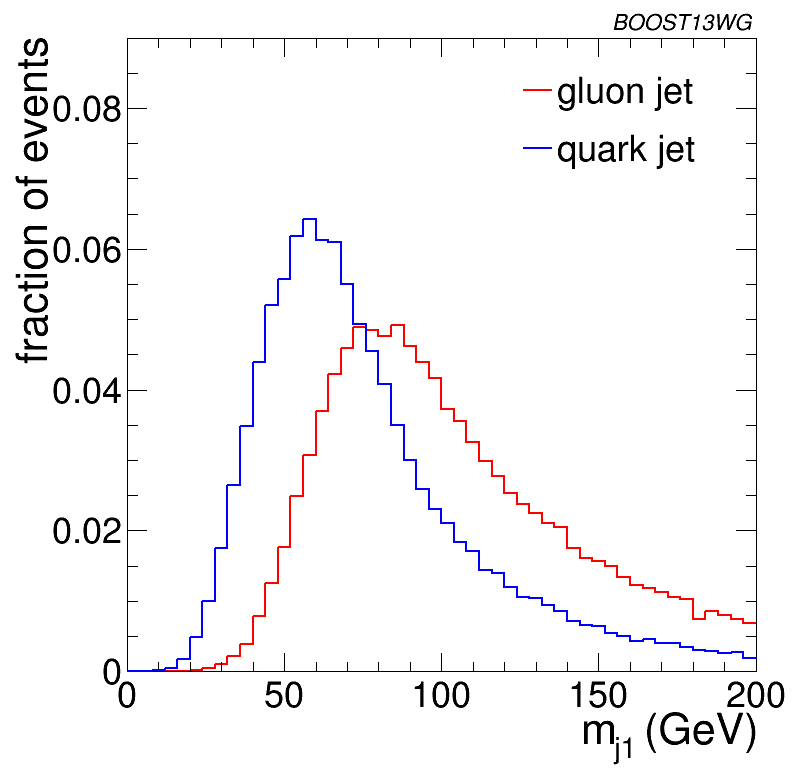
\includegraphics[width=0.30\textwidth]{./Figures/QGTagging/pT500/AKtR08/jmass1.png}}
%\subfigure[Pruned mass]{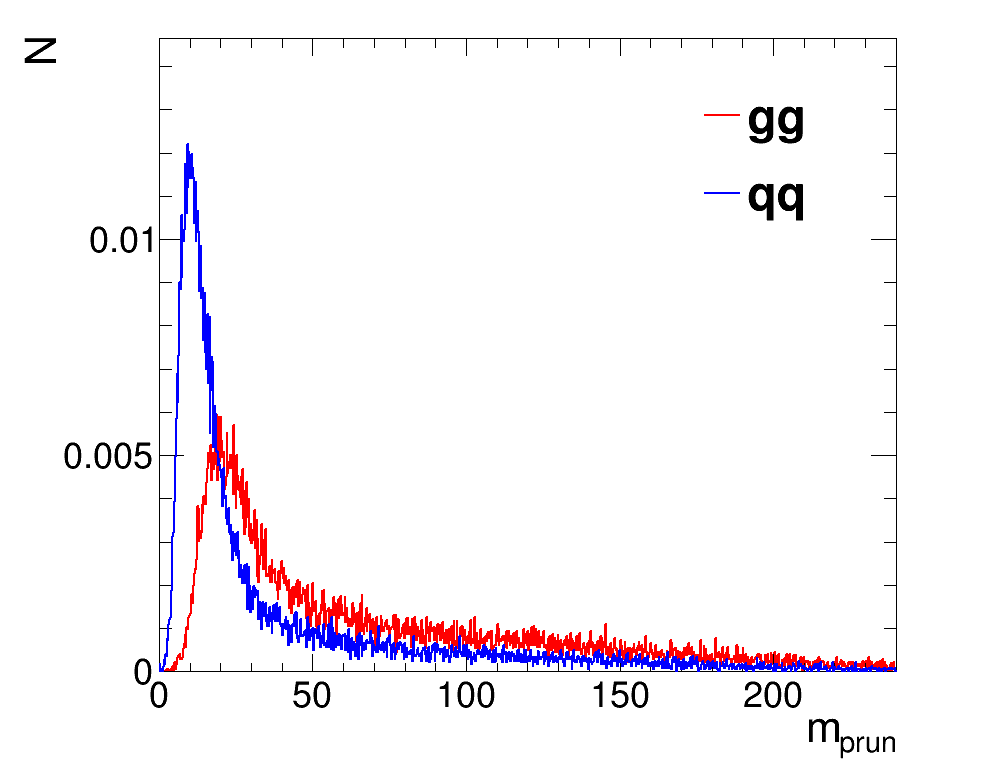
\includegraphics[width=0.30\textwidth]{./Figures/QGTagging/pT500/AKtR08/h_mass_prun.png}}
%\subfigure[Trimmed mass]{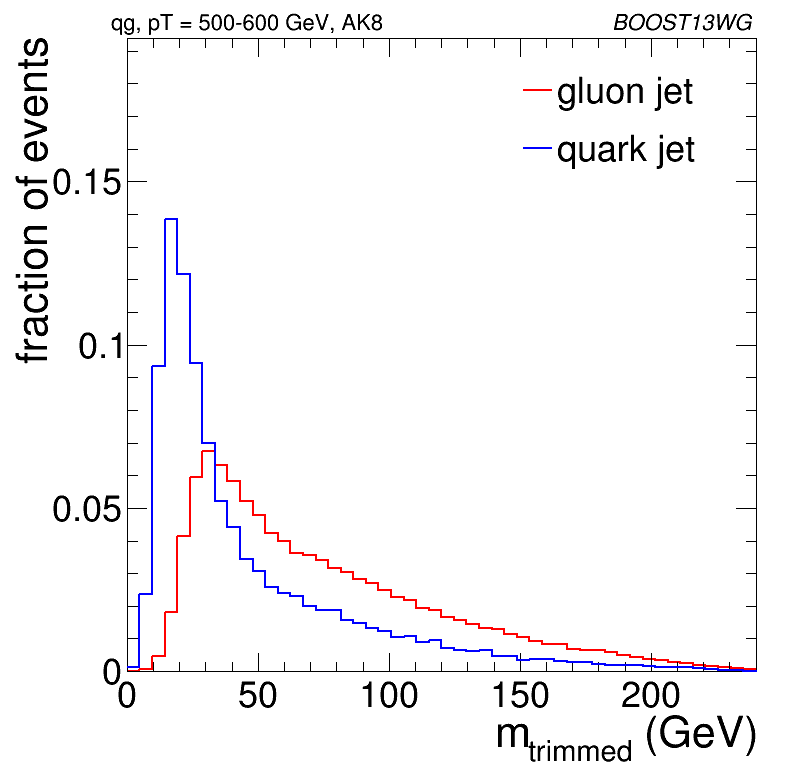
\includegraphics[width=0.30\textwidth]{./Figures/QGTagging/pT500/AKtR08/h_mass_trim.png}}\\
%\subfigure[mMDT mass]{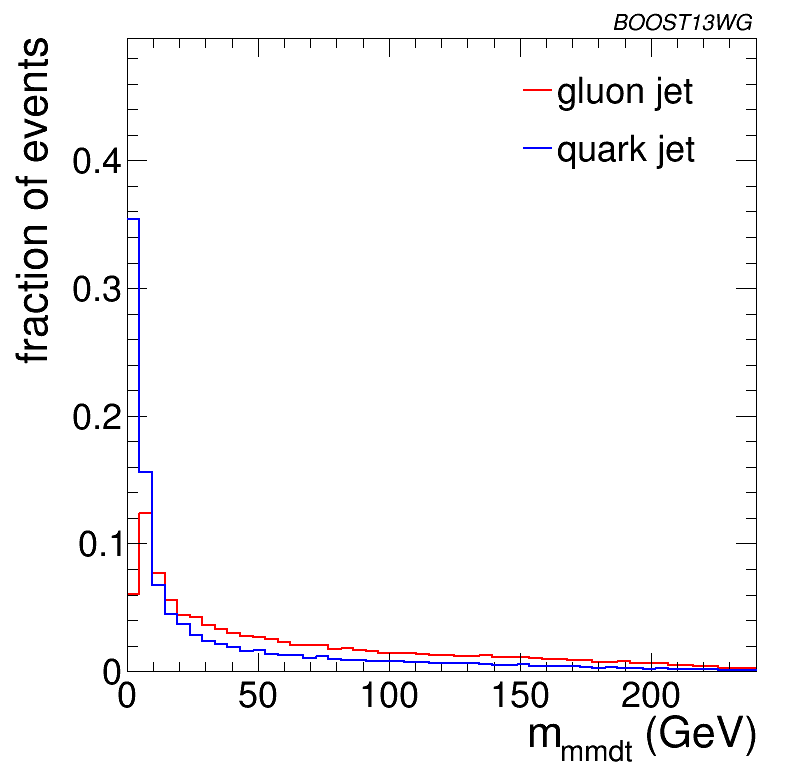
\includegraphics[width=0.30\textwidth]{./Figures/QGTagging/pT500/AKtR08/h_mass_mmdt.png}}
%\subfigure[Soft-drop $\beta=2$ mass]{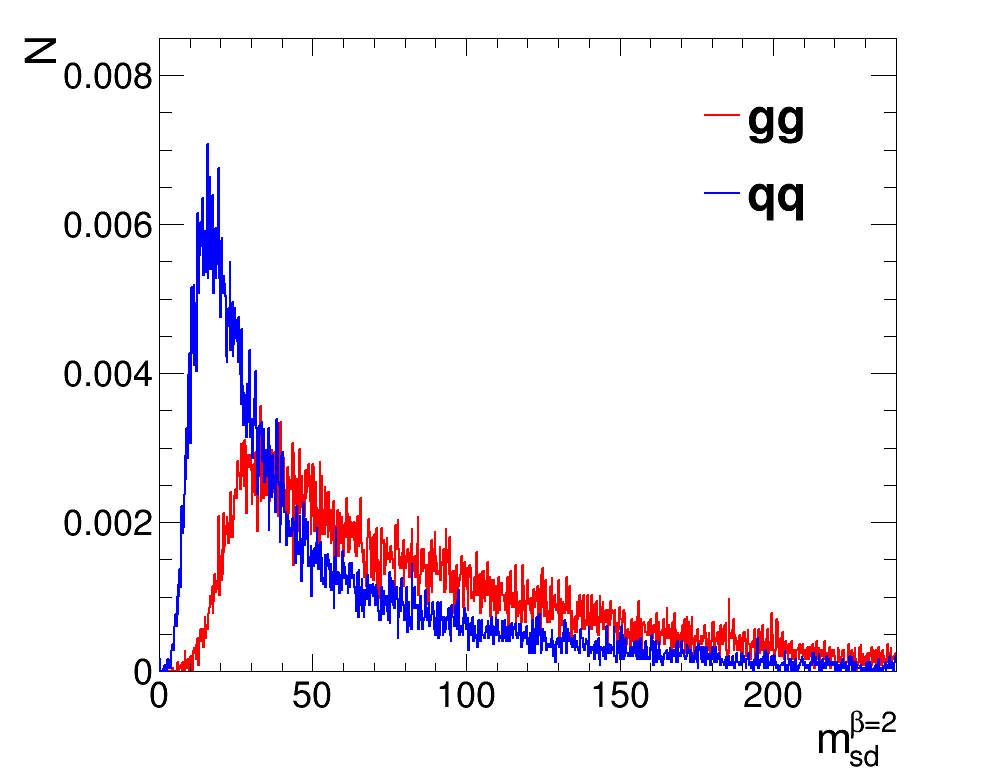
\includegraphics[width=0.30\textwidth]{./Figures/QGTagging/pT500/AKtR08/h_mass_sdb2.png}}
%\subfigure[Soft-drop $\beta=-1$ mass]{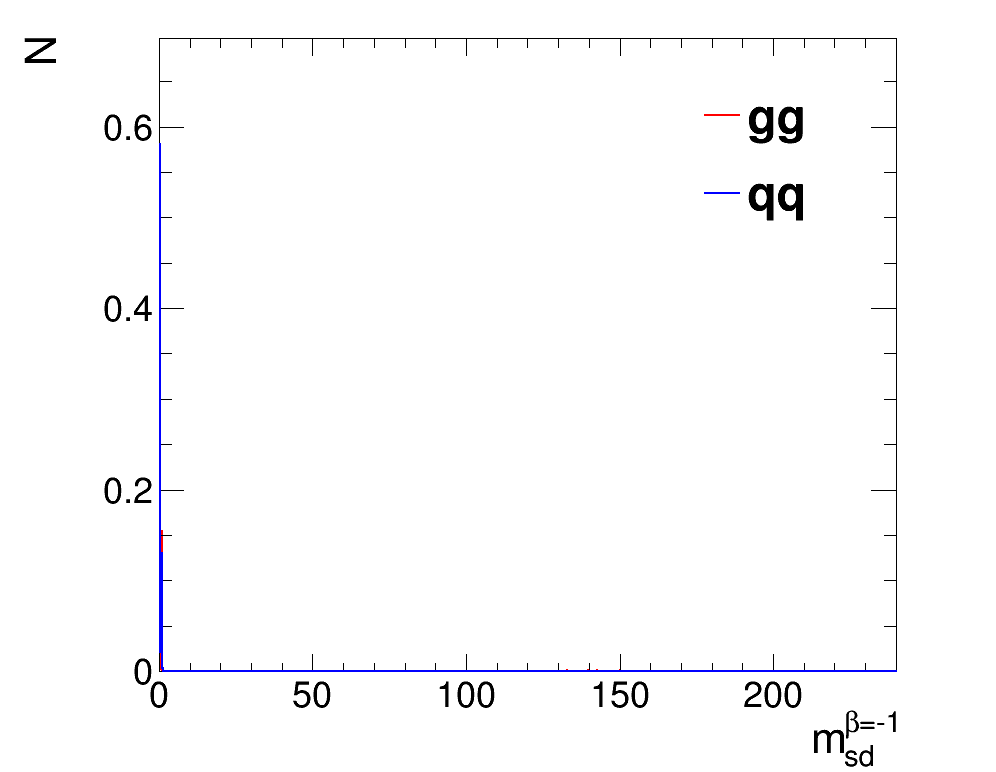
\includegraphics[width=0.30\textwidth]{./Figures/QGTagging/pT500/AKtR08/h_mass_sdm1.png}}
%\caption{Comparisons of ungroomed and groomed quark and gluon mass distributions for leading jets in the 
%$\pt=500-600 \GeV$ bin using the anti-\kT R=0.8 algorithm. }
%\label{fig:qg_pt500_mass_AKt_R08}
%\end{figure*}
%Qualitatively, the application of grooming shifts the mass distributions towards
%lower values when compared to the ungroomed mass, as expected. No clear gain in discrimination can be seen, and for
%certain grooming parameters, such as the use of soft drop with $\beta=-1$ a clear
%loss in discrimination power is observed; this is because the soft-drop condition for $\beta=-1$ discards collinear radiation, and the differences between quarks %and gluons are manifest in the collinear structure (spin, splitting functions, etc.). 


\begin{figure*}
\centering
\subfigure[$\rm{N_ {constits}}$]{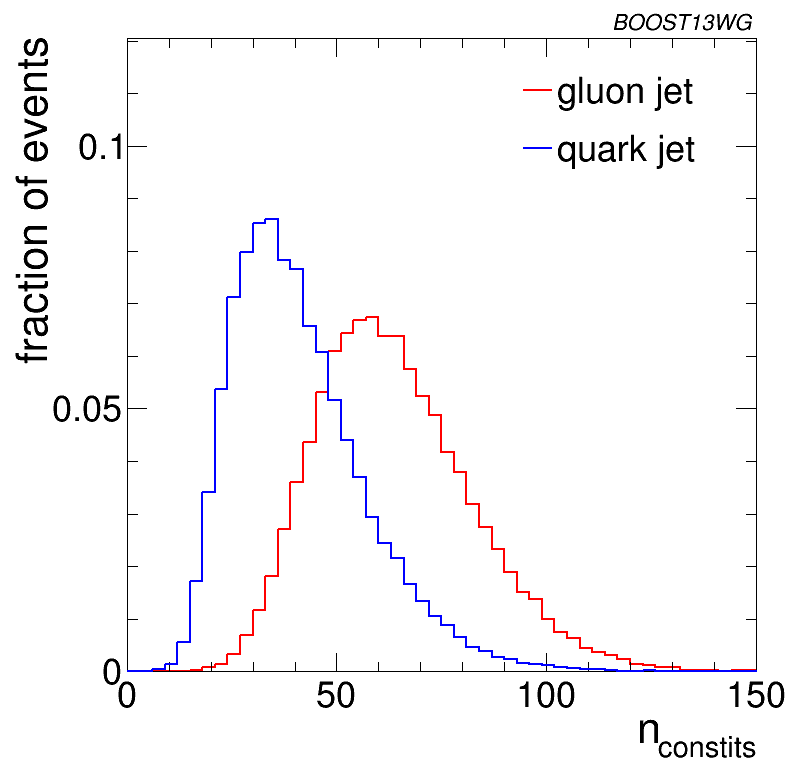
\includegraphics[width=0.30\textwidth]{./Figures/QGTagging/pT500/AKtR08/h_multiplicity.png}}
\subfigure[$\Gamma_{Qjet}$]{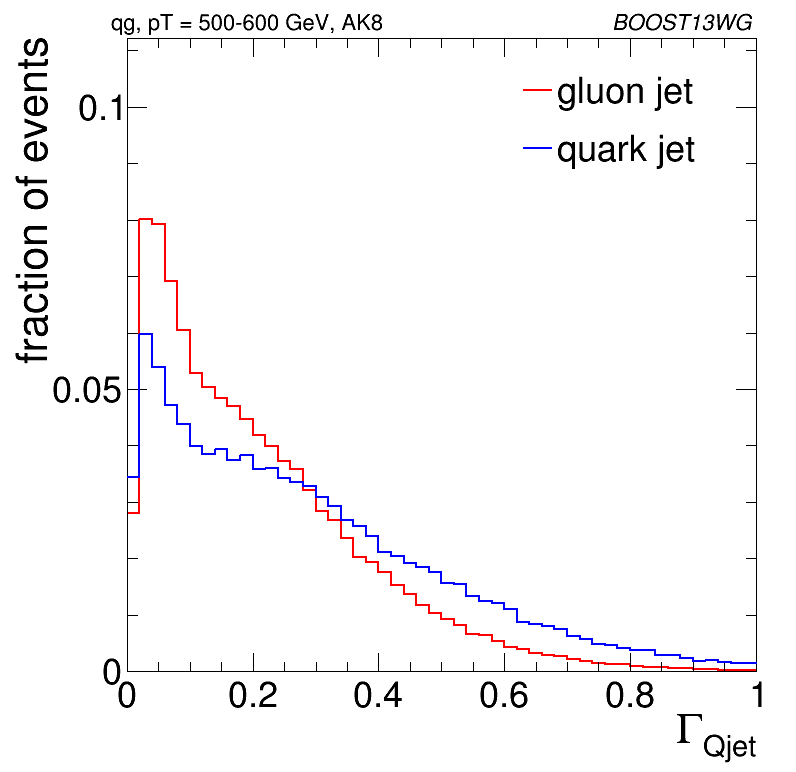
\includegraphics[width=0.30\textwidth]{./Figures/QGTagging/pT500/AKtR08/h_qjetVol.png}}
\subfigure[$C_1^{\beta=0}$]{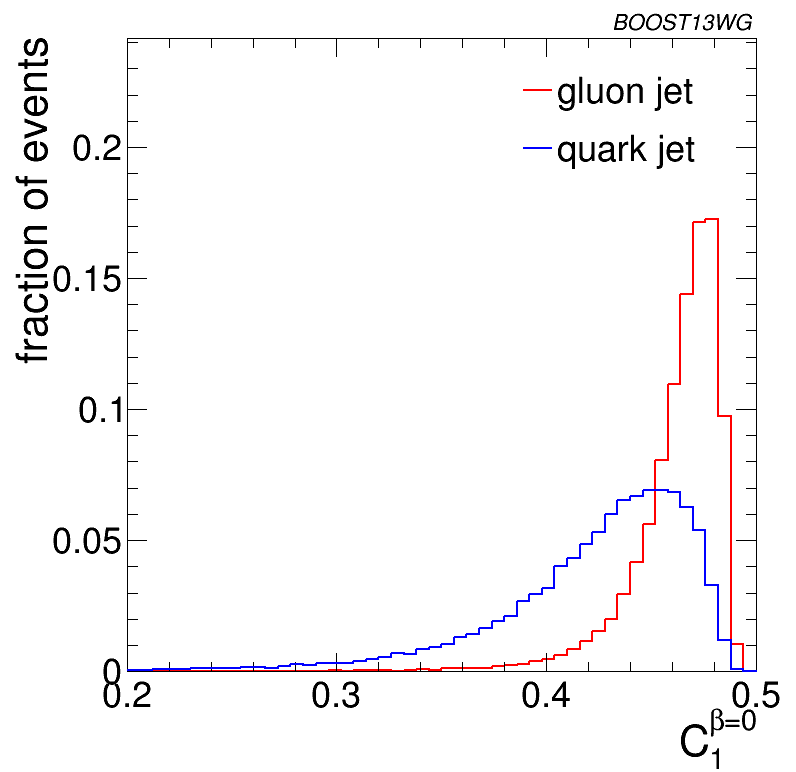
\includegraphics[width=0.30\textwidth]{./Figures/QGTagging/pT500/AKtR08/h_c1_b0.png}}\\
\subfigure[$C_1^{\beta=1}$]{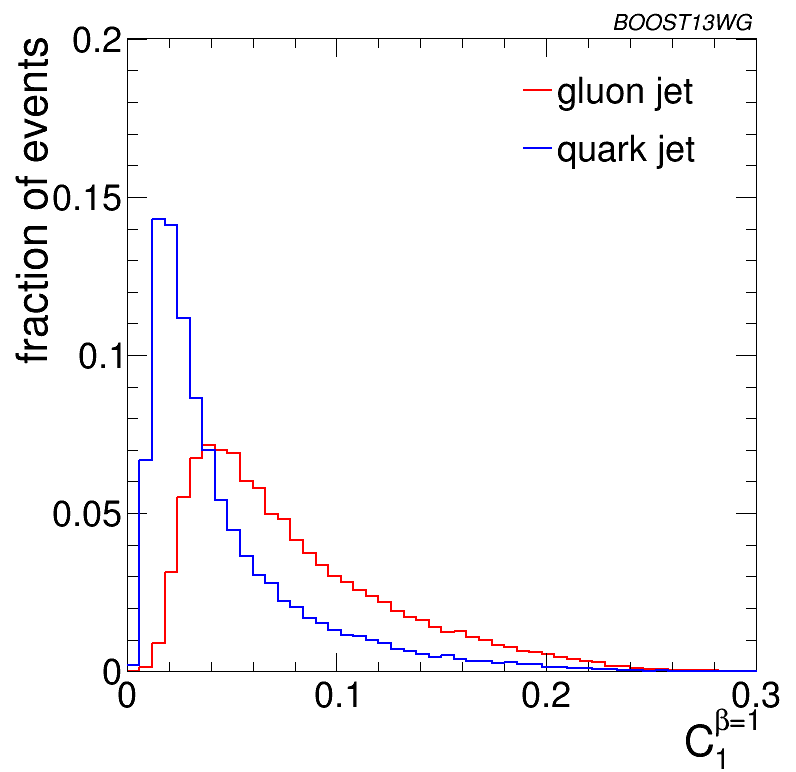
\includegraphics[width=0.30\textwidth]{./Figures/QGTagging/pT500/AKtR08/h_c1_b1.png}}
\subfigure[$\tau_{1}^{\beta=1}$]{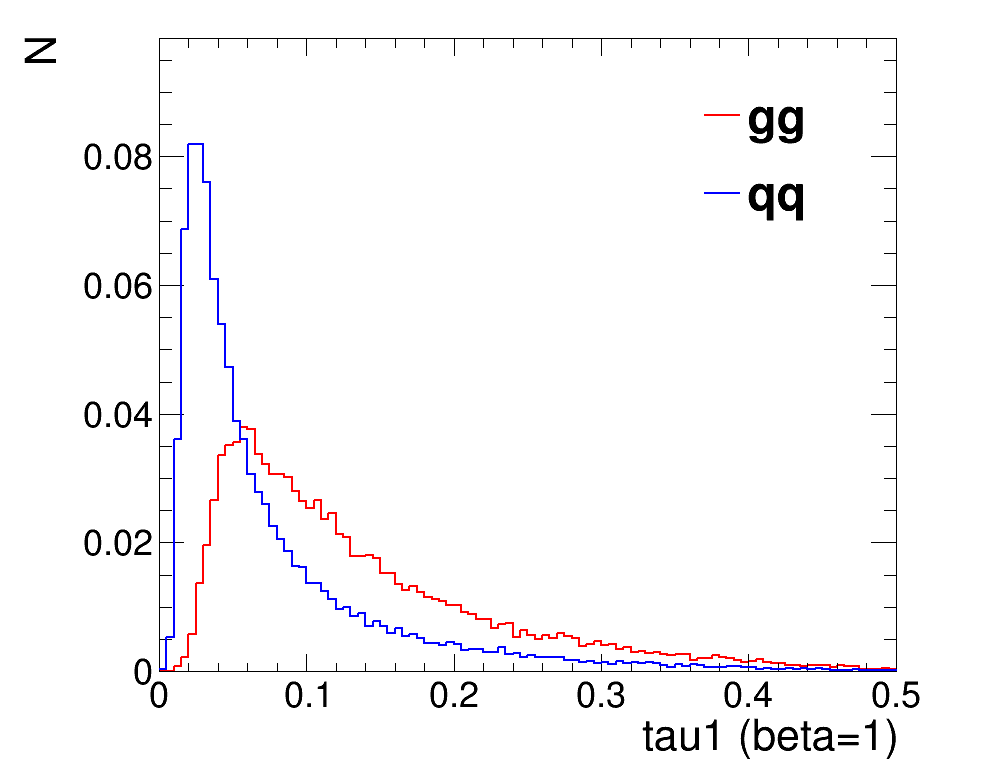
\includegraphics[width=0.30\textwidth]{./Figures/QGTagging/pT500/AKtR08/h_tau1_b1.png}}\\
\subfigure[$C_1^{\beta=2}$]{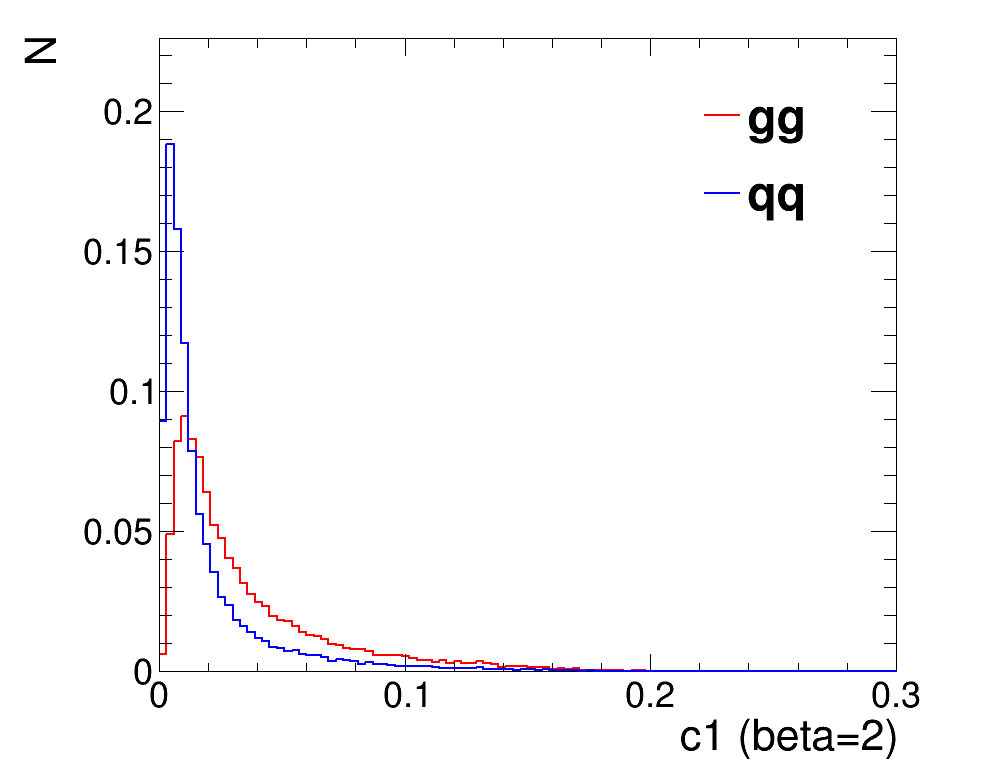
\includegraphics[width=0.30\textwidth]{./Figures/QGTagging/pT500/AKtR08/h_c1_b2.png}}
\subfigure[$\tau_{1}^{\beta=2}$]{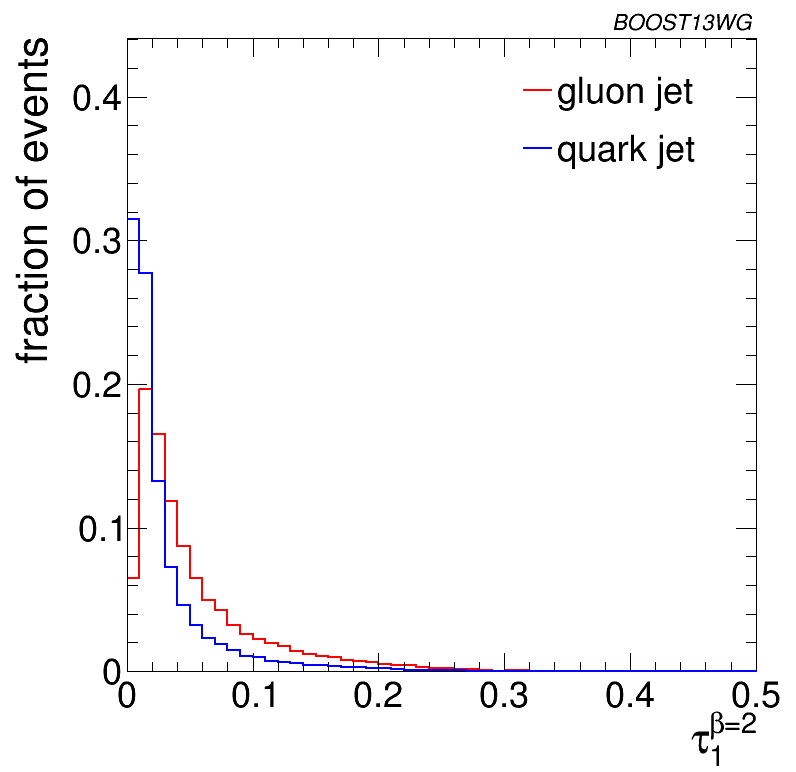
\includegraphics[width=0.30\textwidth]{./Figures/QGTagging/pT500/AKtR08/h_tau1_b2.png}}
\subfigure[Ungroomed mass]{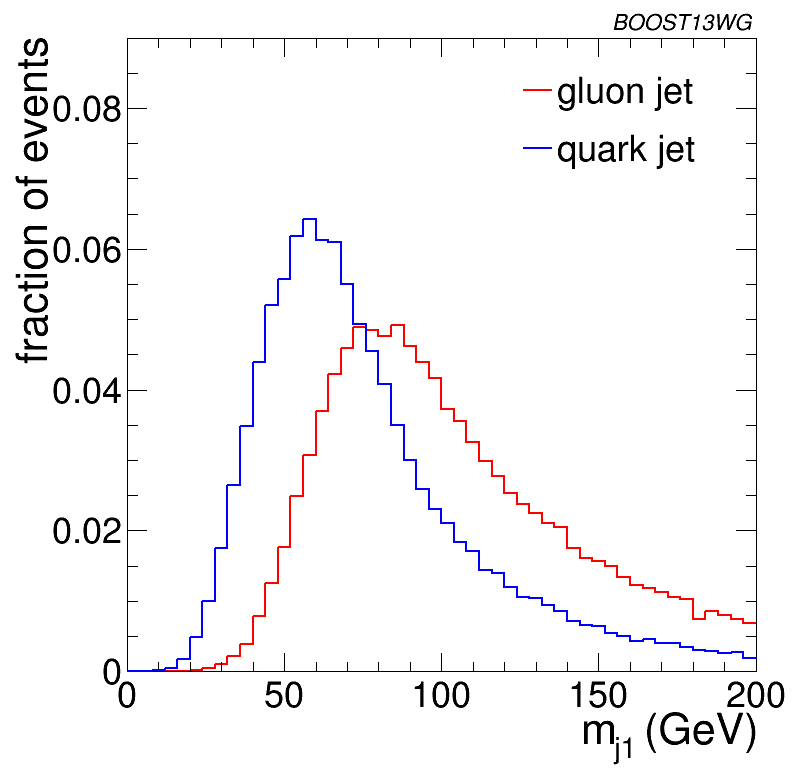
\includegraphics[width=0.30\textwidth]{./Figures/QGTagging/pT500/AKtR08/jmass1.png}}
\caption{Comparisons of quark and gluon distributions of different substructure variables (organized by Class) for leading jets in the 
$\pt=500-600 \GeV$ bin using the anti-\kT $R=0.8$ algorithm. }
\label{fig:qg_pt500_subst_AKt_R08}
\end{figure*}

The quark and gluon distributions of different substructure observables
are shown in Figure~\ref{fig:qg_pt500_subst_AKt_R08}, which already illustrates at least some of the points about the Classes made above. 
At a fundamental level the primary difference between quark jets and gluon jets is the color charge of the initiating parton, typically expressed in terms of the
ratio of the corresponding Casimir factors $C_F/C_A = 4/9$.  Since the quark has the smaller color charge, it will radiate less than a corresponding
gluon and the resulting jet will contain fewer constituents. This difference is clearly indicated in Figure~\ref{fig:qg_pt500_subst_AKt_R08}(a), 
suggesting that simply counting constituents will provide good separation between quark and gluon jets.  In fact, among the observables
considered, one can see by eye that $N_{\rm constits}$ should provide the highest separation
power, \textit{i.e.}, the quark and gluon distributions are most distinct, as was originally noted in \cite{Gallicchio:2011xq,Gallicchio:2012ez}. 
Figure~\ref{fig:qg_pt500_subst_AKt_R08} further suggests
that $C_1^{\beta=0}$ should provide the next best separation followed by $C_1^{\beta=1}$, as was also
found by the CMS and ATLAS Collaborations\cite{Aad:2014gea}.   

To more quantitatively study the power of each observable as a
discriminator for quark/gluon tagging, ROC curves are built by scanning each distribution
and plotting the background efficiency (to select gluon jets) vs.~the signal efficiency (to select quark jets). 
Figure~\ref{fig:qg_pt300_single} shows these ROC curves for all of the
substructure variables shown in 
Figure~\ref{fig:qg_pt500_subst_AKt_R08}, along with the ungroomed mass, representing the 
best performing mass variable, for R=0.4, 0.8 and 1.2 jets in the $\pt=300-400\GeV$
bin. In addition, the ROC curve for a tagger built from a BDT
combination of all the variables (see Section~\ref{sec:multivariate}) is shown.
%
\begin{figure*}
\centering
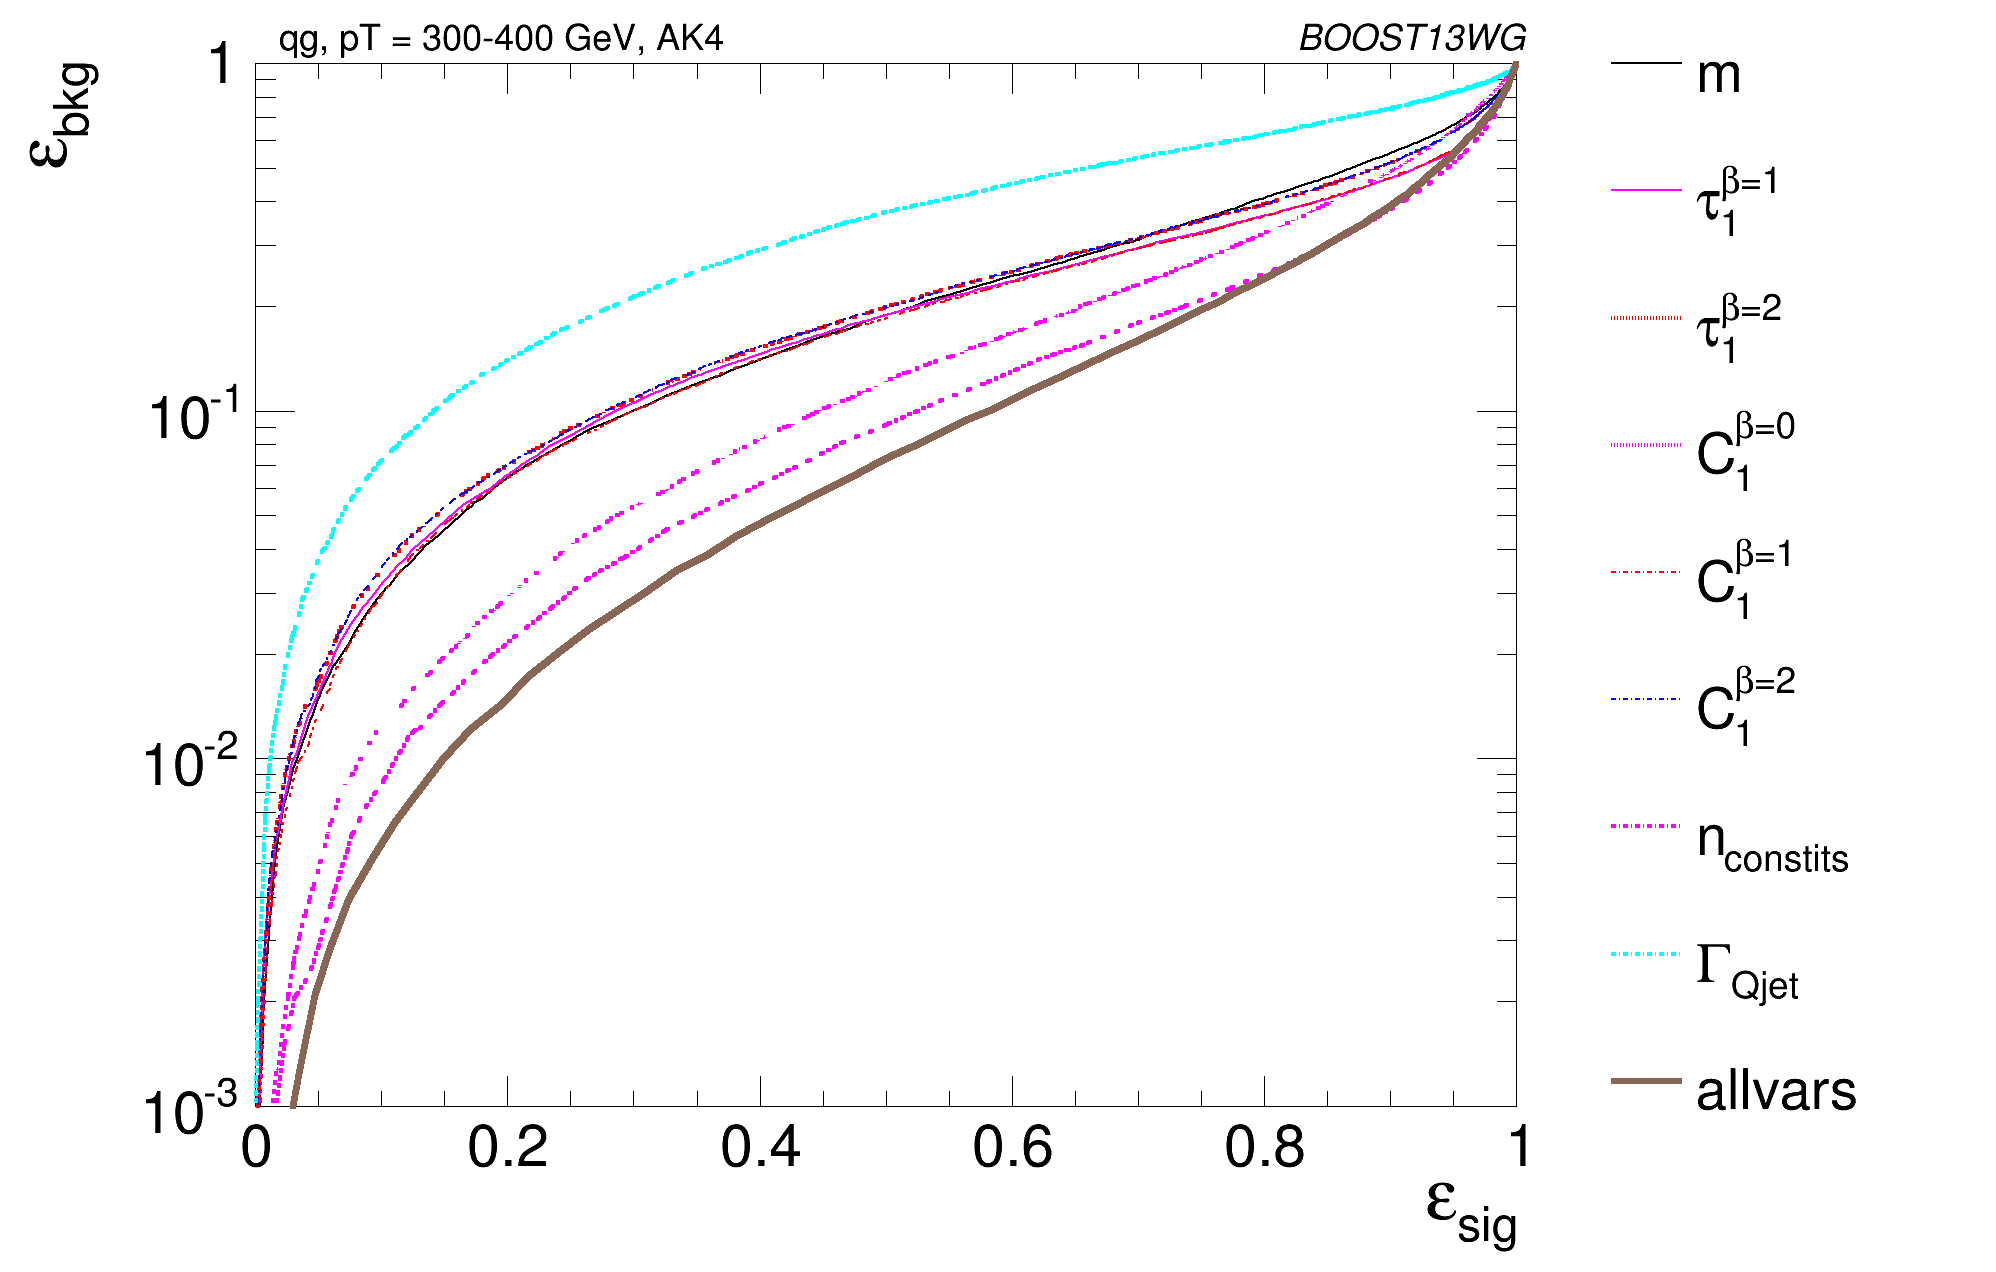
\includegraphics[width=0.48\textwidth]{./Figures/QGTagging/pT300/AKtR04/Rocs_1D_single.png}
%\includegraphics[width=0.4\textwidth]{./Figures/QGTagging/pT1000/AKtR04/Rocs_1D_single.png}\\
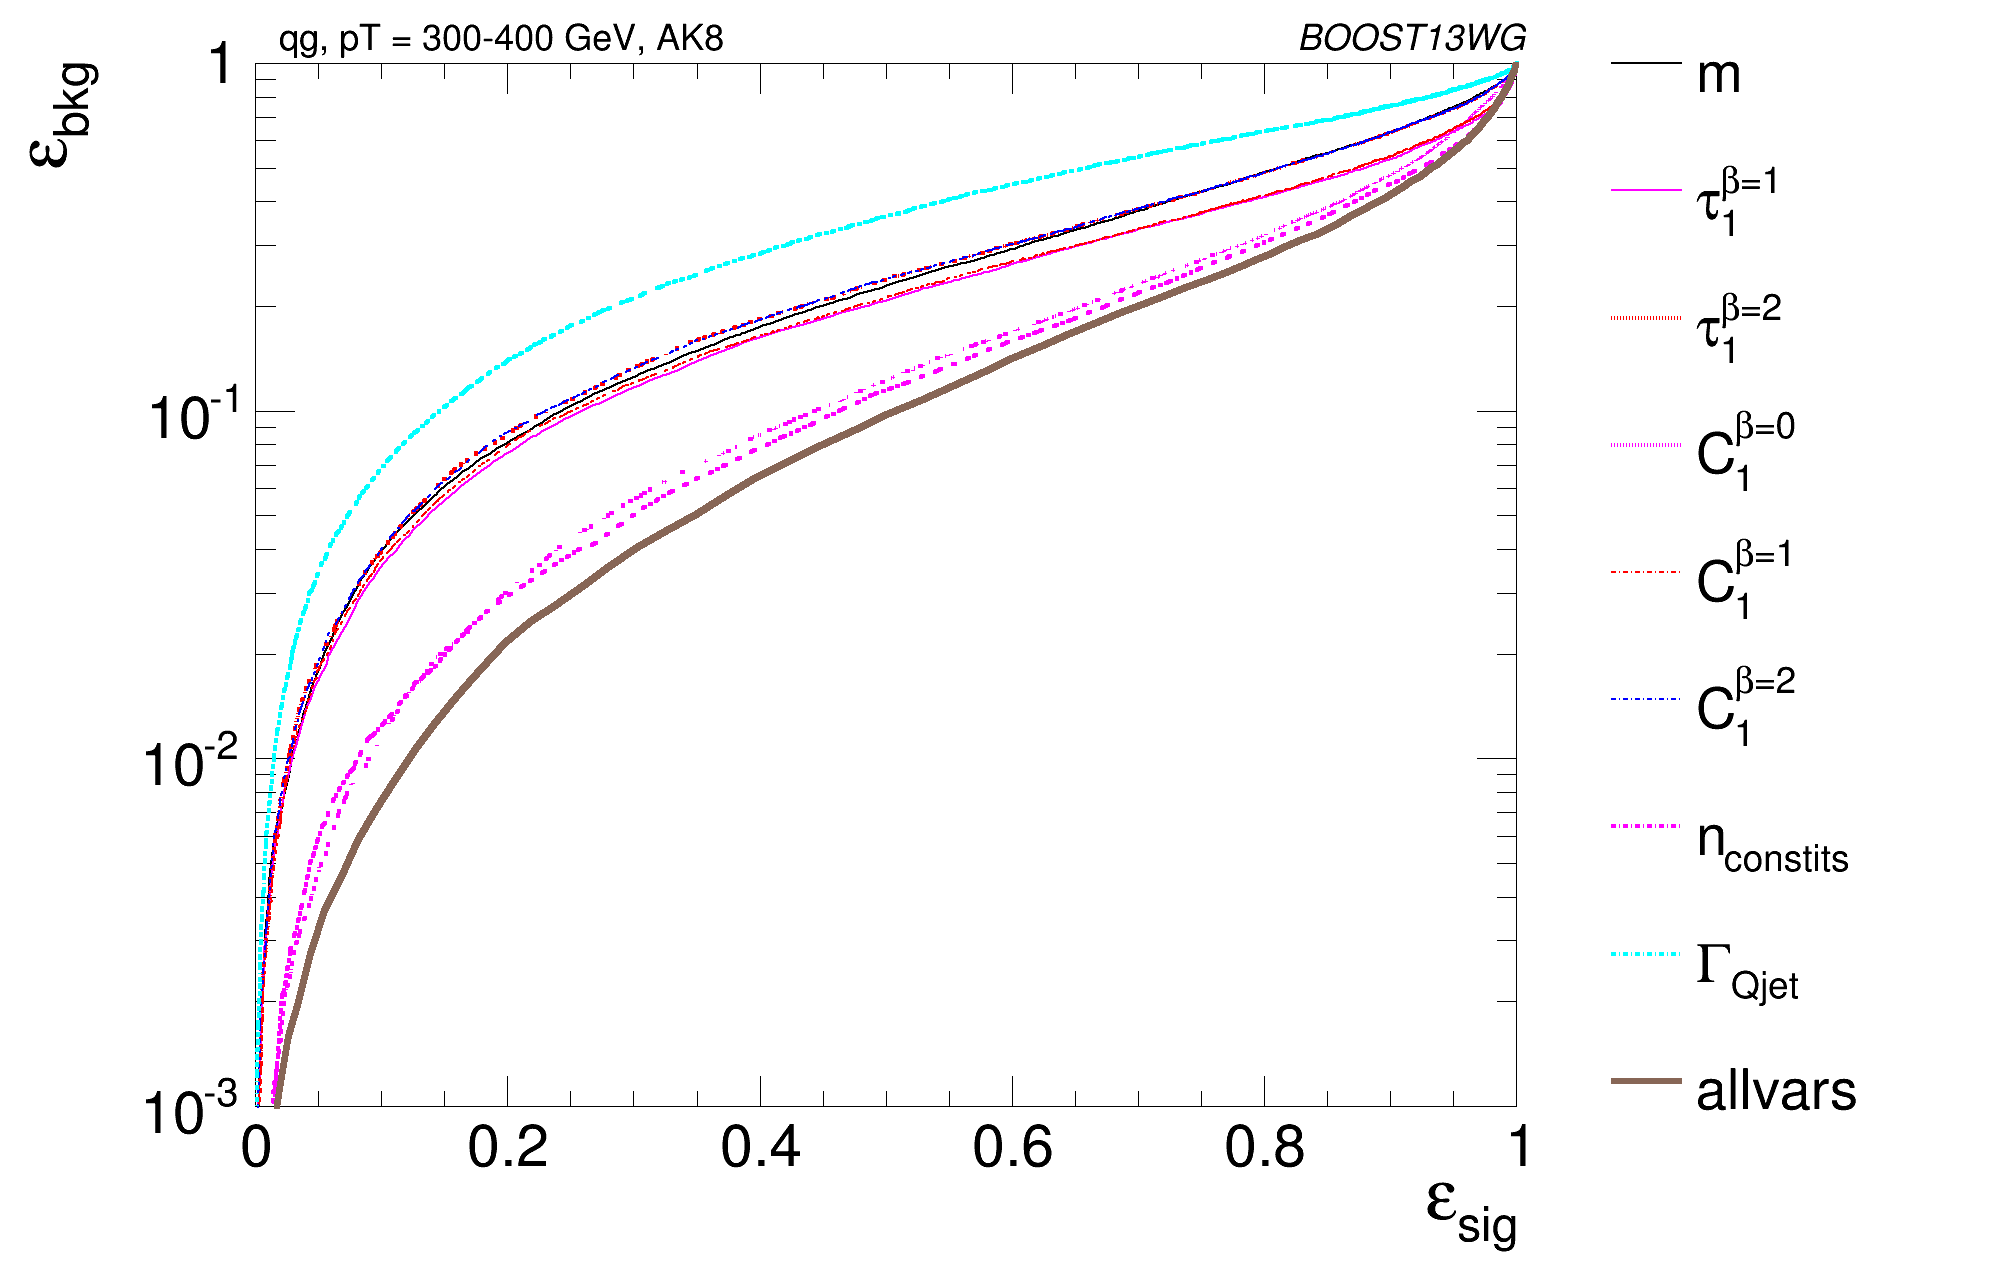
\includegraphics[width=0.48\textwidth]{./Figures/QGTagging/pT300/AKtR08/Rocs_1D_single.png}
%\includegraphics[width=0.4\textwidth]{./Figures/QGTagging/pT1000/AKtR08/Rocs_1D_single.png}\\
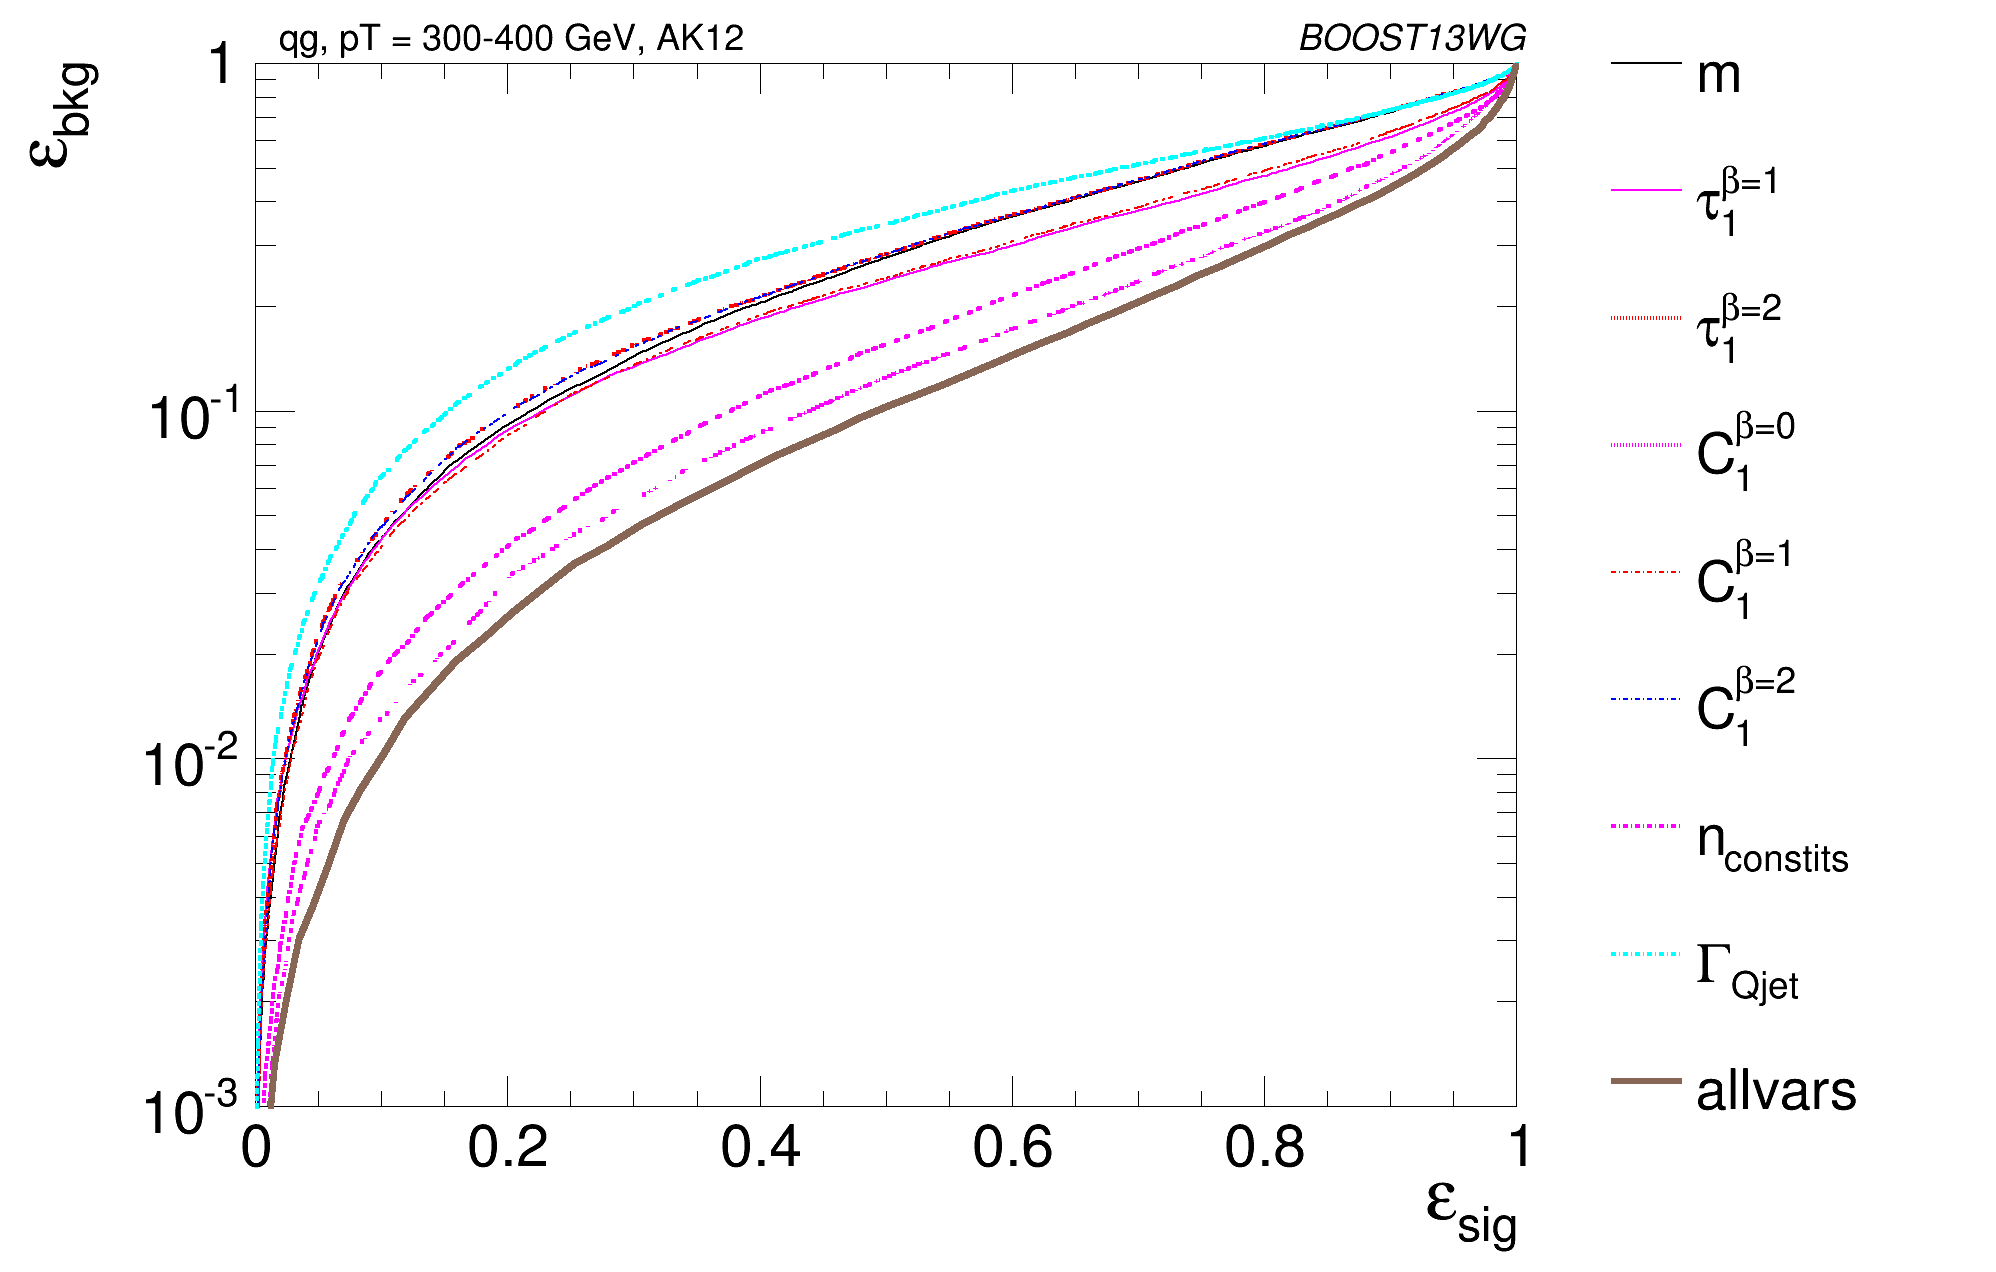
\includegraphics[width=0.48\textwidth]{./Figures/QGTagging/pT300/AKtR12/Rocs_1D_single.png}
%\includegraphics[width=0.4\textwidth]{./Figures/QGTagging/pT1000/AKtR12/Rocs_1D_single.png}\\
\caption{The ROC curve for all single variables considered for
  quark-gluon discrimination in the \pt 300-400 GeV bin using the
  anti-\kT R=0.4, 0.8 and 1.2 algorithm.%{\bf ED: Hard to tell the lines on the plots apart}
}
\label{fig:qg_pt300_single}
\end{figure*}
%
Clearly, and as suggested earlier, $n_{\rm constits}$ is the best performing variable for all Rs, even though $C_1^{\beta=0}$ is close, particularly
for R=0.8. Most other variables have similar performance, except $\Gamma_{\rm Qjet}$, which shows significantly worse
discrimination (this may be due to our choice of
rigidity $\alpha = 0.1$, with other studies suggesting that a smaller value,
such as $\alpha = 0.01$, produces better results\cite{Ellis:2012sn,Ellis:2014eya}). The combination of all variables shows somewhat better discrimination, and
we will discuss in more detail below the correlations between the observables and their impact on the combined discrimination power.

%
\begin{figure*}
\centering
\subfigure[$\rm{N_ {constits}}$]{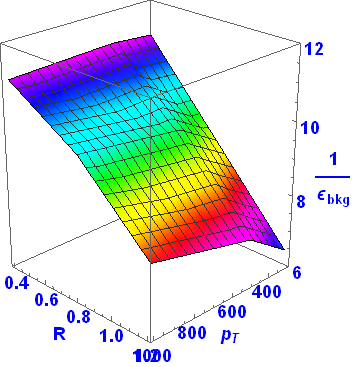
\includegraphics[width=0.30\textwidth]{./Figures/QGSurface/Ncon.png}}
\subfigure[$\Gamma_{Qjet}$]{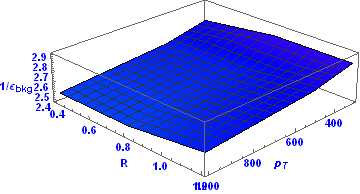
\includegraphics[width=0.30\textwidth]{./Figures/QGSurface/GamQ.png}}
\subfigure[$C_1^{\beta=0}$]{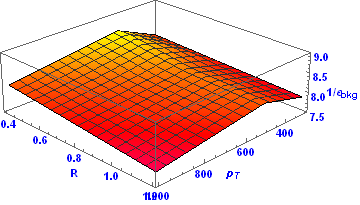
\includegraphics[width=0.30\textwidth]{./Figures/QGSurface/C10.png}}\\
\subfigure[$C_1^{\beta=1}$]{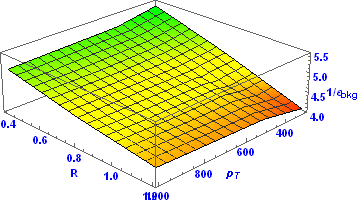
\includegraphics[width=0.30\textwidth]{./Figures/QGSurface/C11.png}}
\subfigure[$\tau_{1}^{\beta=1}$]{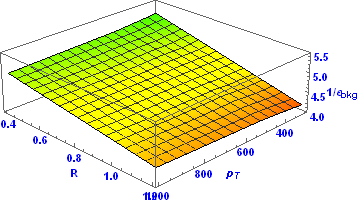
\includegraphics[width=0.30\textwidth]{./Figures/QGSurface/Tau11.png}}\\
\subfigure[$C_1^{\beta=2}$]{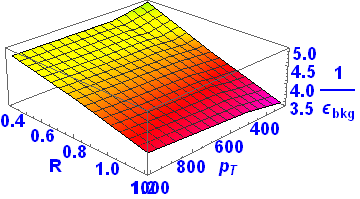
\includegraphics[width=0.30\textwidth]{./Figures/QGSurface/C12.png}}
\subfigure[$\tau_{1}^{\beta=2}$]{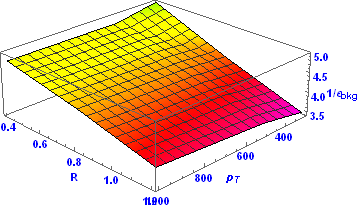
\includegraphics[width=0.30\textwidth]{./Figures/QGSurface/Tau12.png}}
\subfigure[Ungroomed mass]{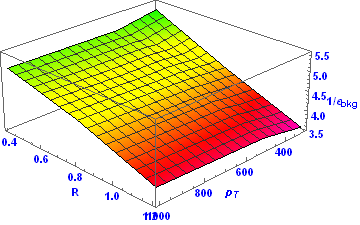
\includegraphics[width=0.30\textwidth]{./Figures/QGSurface/Mass.png}}\\
\caption{Surface plots of $1/\epsilon_\text{bkg}$ for all single variables considered for
  quark-gluon discrimination as functions of $R$ and $\pt$. }
\label{fig:qg_surface_single}
\end{figure*}
%

We now examine how the performance of the substructure observables changes with $\pt$ and $R$.  To present the results in a ``digestible'' fashion
we will focus on the gluon jet ``rejection'' factor, $1/\epsilon_\text{bkg}$, for a quark signal efficiency, $\epsilon_\text{sig}$, of $50\,\%$.
We can use the values of $1/\epsilon_\text{bkg}$ generated for the 9 kinematic points introduced above ($R = 0.4, 0.8, 1.2$ and 
the 100 GeV $\pt$ bins with lower limits
$p_T = 300\, \text{GeV}$, $500\, \text{GeV}$, $1000\,\text{GeV}$) to generate surface plots.  The surface plots in Figure~\ref{fig:qg_surface_single}
indicate both the level of gluon rejection
and the variation with $\pt$ and $R$ for each of the studied single observable.  The color shading is defined so that a change in color 
corresponds to a change of about 0.4 in $1/\epsilon_\text{bkg}$.  The colors have the same correlation with the magnitude of $1/\epsilon_\text{bkg}$
in all of the plots, but repeat after a change of about 4.  Thus ``blue'' corresponds to a value of about 2.5 in  Figure~\ref{fig:qg_surface_single}(b) and the
values 6.5 and 10.5
in  Figure~\ref{fig:qg_surface_single}(a), while ''yellow'' corresponds to about 5 in  Figures~\ref{fig:qg_surface_single}(c) to (h) and about 9 in
 Figure~\ref{fig:qg_surface_single}(a).

We see, as expected, that the numerically largest rejection rates occur
for the observable $N_{\rm constits}$ in  Figure~\ref{fig:qg_surface_single}(a), where the rejection factor is in the range 6 to 11 and 
varies rather dramatically with $R$.  As $R$ increases the jet collects more constituents from the underlying event, which are the same
for quark and gluon jets, and the separation power decreases.  At large $R$, there is some improvement with increasing $\pt$ due to the 
enhanced radiation, which does distinguish quarks from gluons.  Figure~\ref{fig:qg_surface_single}(b) confirms the limited efficacy of the single
observable $\Gamma_{Qjet}$ (at least for our parameter choices) with a rejection rate only in the range 2.5 to 2.8.  On the other hand, this 
observable probes a very different
property of jet substructure, \textit{i.e.}, the sensitivity to detailed changes in the grooming procedure, and this difference is suggested
by the distinct $R$ and $\pt$ dependence illustrated in  Figure~\ref{fig:qg_surface_single}(b).  The rejection rate increases with increasing $R$
and decreasing $\pt$, since the distinction between quark and gluon jets for this observable arises from the relative importance of the one
``hard'' gluon emission configuration.  The role of this contribution is enhanced for both decreasing $\pt$ and increasing $R$. 
Figure~\ref{fig:qg_surface_single}(c) indicates that the observable $C_1^{\beta=0}$ can, by itself, provide a rejection rate in the range
7.8 to 8.6 (intermediate between the two previous observables) and again with distinct $R$ and $\pt$ dependence.  In this case the rejection
rate decreases slowly with increasing $R$ ($\beta = 0$ explicitly means that the angular dependence is much reduced), 
while the rejection rate peaks at intermediate $\pt$ values (an effect visually enhanced by the limited number of 
$\pt$ values included).  Both the distinct values of the rejection rates and the differing $R$ and $\pt$ dependence serve to confirm that these three
observables tend to probe independent features of the quark and gluon jets.  

Figures~\ref{fig:qg_surface_single}(d) and (e) serve to confirm
the very similar properties of the Class IV observables $C_1^{\beta=1}$ and $\tau_1^{\beta=1}$ (as already suggested in
Figures~\ref{fig:qg_pt500_subst_AKt_R08}(d) and (e))
with essentially identical rejection rates (4.1 to 5.4) and identical $R$ and $\pt$ dependence (a slow decrease with increasing $R$ and an even
slower increase with increasing $\pt$).  
A similar conclusion for the Class V observables $C_1^{\beta=2}$, $\tau_1^{\beta=2}$ and $m$ with similar rejection rates in the 
range 3.5 to 5.3 and very similar $R$ and $\pt$ dependence (a slow decrease with increasing $R$ and an even
slower increase with increasing $\pt$).  Arguably, drawing a distinction between the Class IV and Class V observables, is a fine point, 
but the color shading does suggest some
distinction from the slightly smaller rejection rate in Class V.  Again the strong similarities between the plots within the second and third rows in 
Figure~\ref{fig:qg_surface_single} speaks to the common properties of the observables within the two classes.


 
%For jet masses, few variations are observed as the 
%radius parameter of the jet reconstruction is increased in the two highest $\pt$ bins; this is because the radiation
%is more collimated and the dependence on $R$ is consequently smaller.
%However, for the $300-400\GeV$ bin, the use of small-$R$ jets produces a shift in the
%mass distributions towards lower values, so that large-$R$ jet masses are more stable
%with $\pt$ and small-$R$ jet masses are smaller at low-$\pt$ as expected from the spatial
%constraints imposed by the $R$ parameter. These statements are explored more 
%quantitatively later in this section. ({\bf BS: Do we have plots for this?})

%The evolution of some of the substructure variable distributions with $\pt$ and R is less trivial than
%for the jet masses. In particular, changing the $R$ parameter at high $\pt$ changes significantly the $C_a^{\beta}$
%for $\beta>0$ and the $n_{\rm constits}$ distributions, while leaving all other distributions qualitatively unchanged. 
%This is illustrated in Figure~\ref{fig:Rdep_qg_C_pt1000} for $\beta=0$ and $\beta=1$ using $a=1$ in both cases for
%jets with $\pt=1.0-1.1\TeV$. 

 %
%\begin{figure*}
%\centering
%\subfigure[$C_1^{\beta=0}$, $R=0.4$]{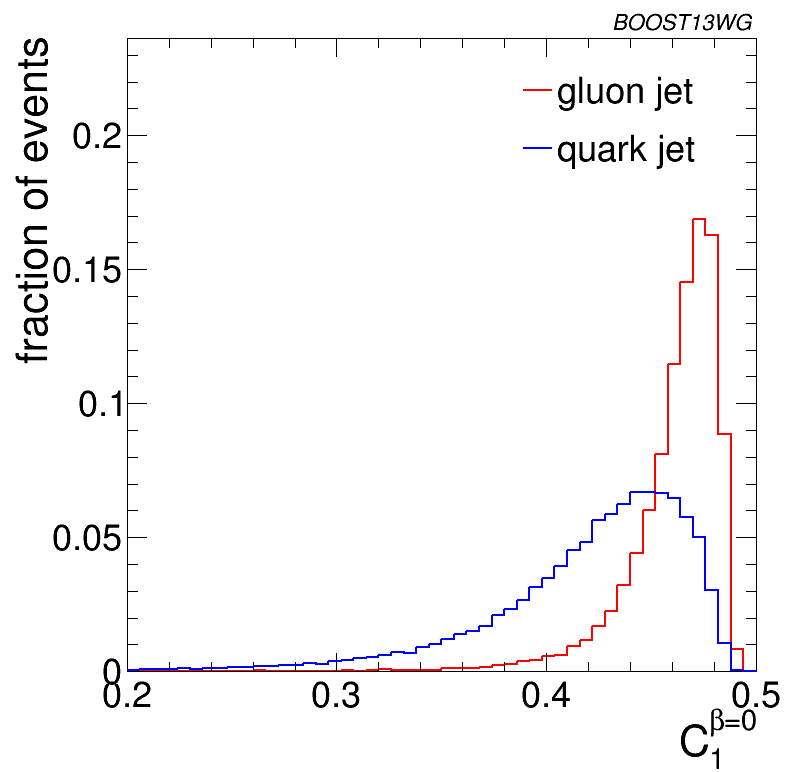
\includegraphics[width=0.30\textwidth]{./Figures/QGTagging/pT1000/AKtR04/h_c1_b0.png}}
%\subfigure[$C_1^{\beta=0}$, $R=0.8$]{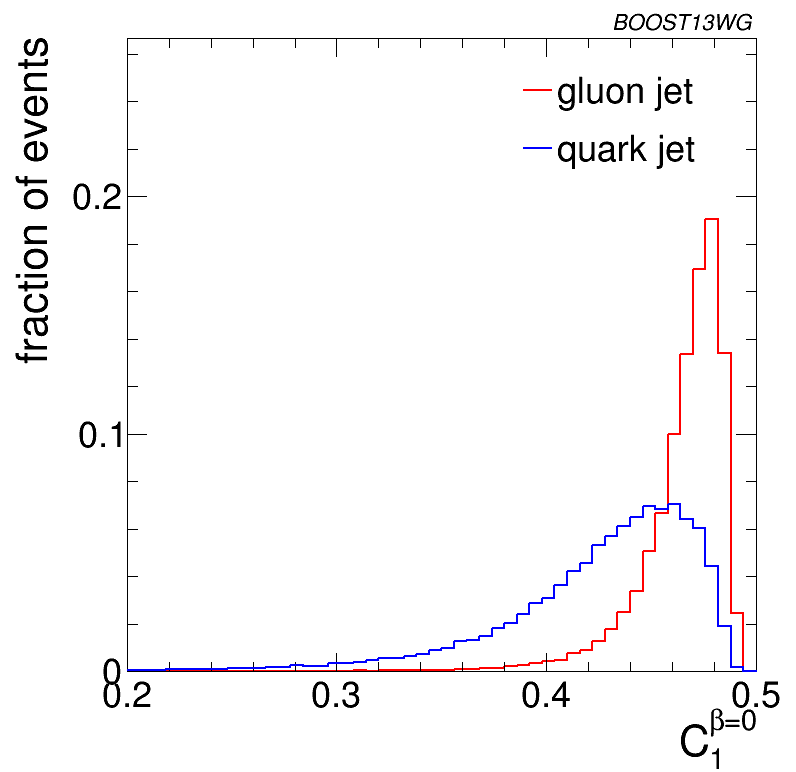
\includegraphics[width=0.30\textwidth]{./Figures/QGTagging/pT1000/AKtR08/h_c1_b0.png}}
%\subfigure[$C_1^{\beta=0}$, $R=1.2$]{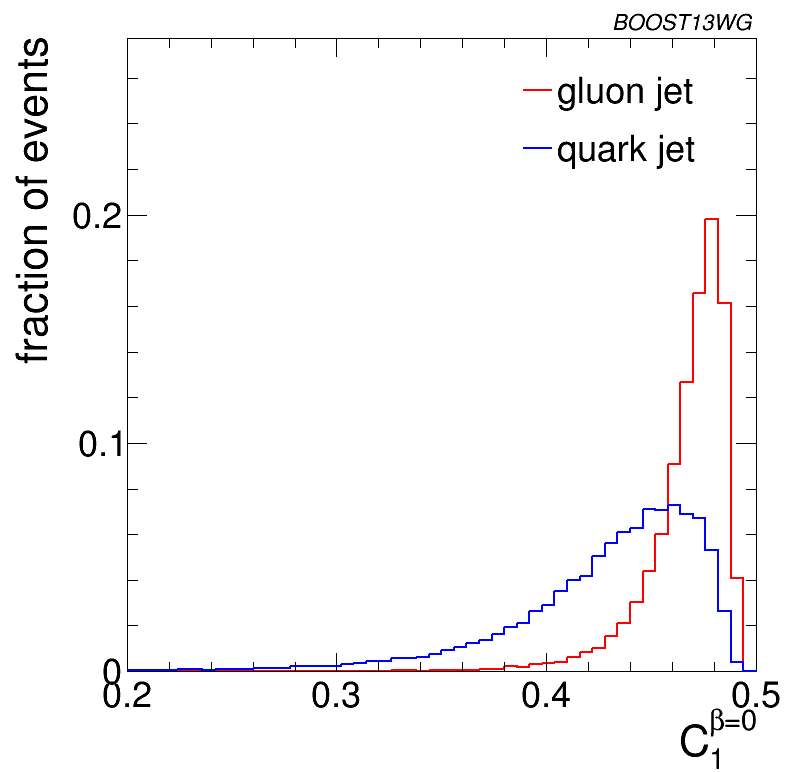
\includegraphics[width=0.30\textwidth]{./Figures/QGTagging/pT1000/AKtR12/h_c1_b0.png}}\\
%\subfigure[$C_1^{\beta=1}$, $R=0.4$]{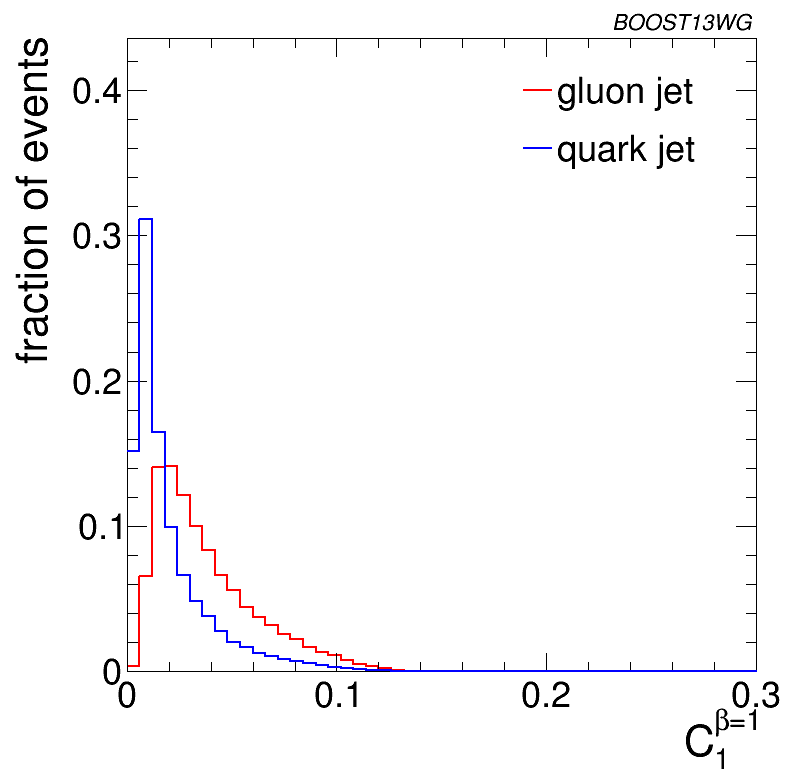
\includegraphics[width=0.30\textwidth]{./Figures/QGTagging/pT1000/AKtR04/h_c1_b1.png}}
%\subfigure[$C_1^{\beta=1}$, $R=0.8$]{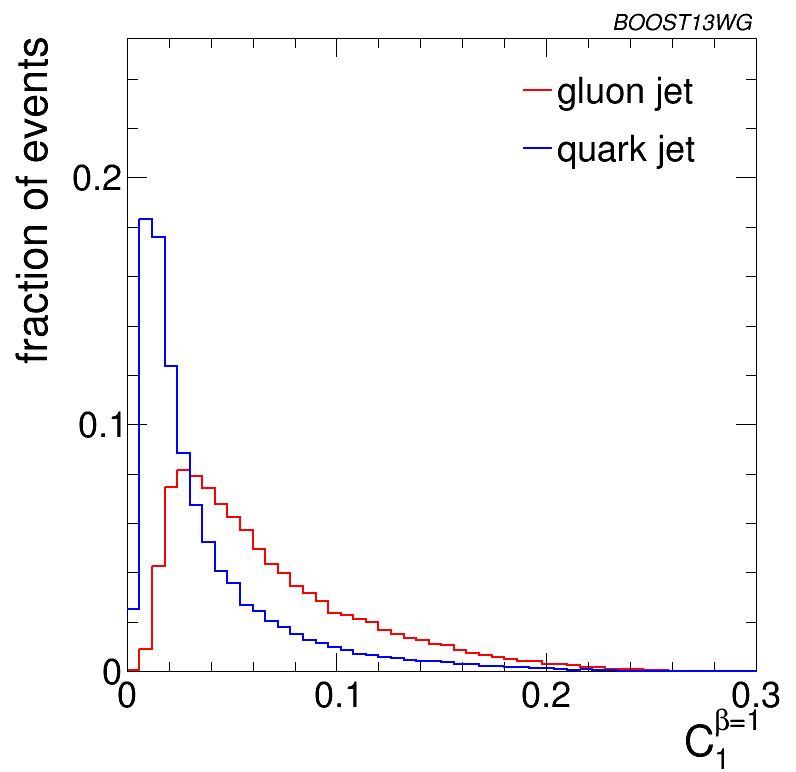
\includegraphics[width=0.30\textwidth]{./Figures/QGTagging/pT1000/AKtR08/h_c1_b1.png}}
%\subfigure[$C_1^{\beta=1}$, $R=1.2$]{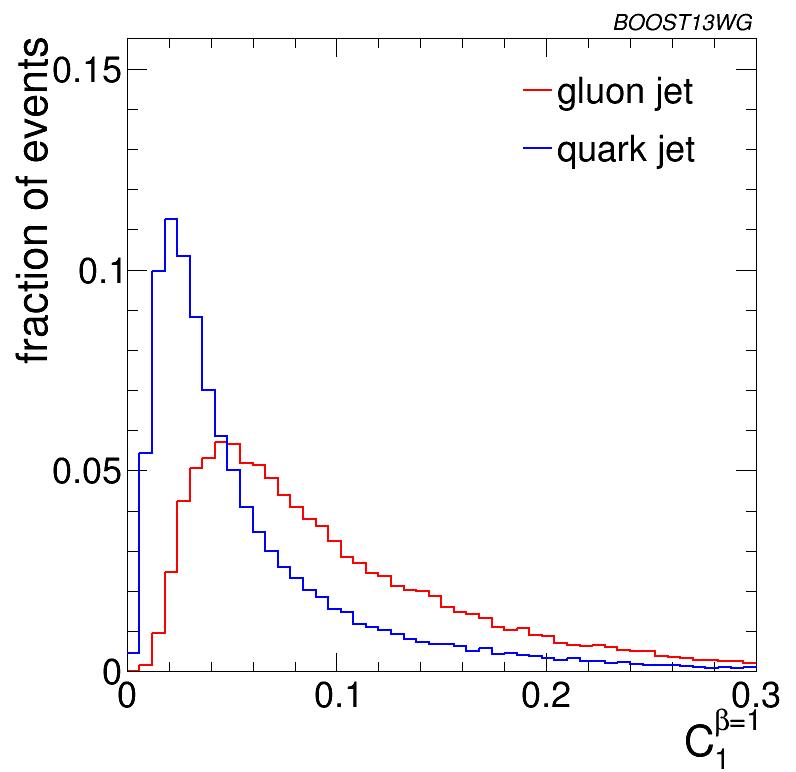
\includegraphics[width=0.30\textwidth]{./Figures/QGTagging/pT1000/AKtR12/h_c1_b1.png}}\\
%\caption{Comparisons of quark and gluon distributions of $C_1^{\beta=0}$ (top) and $C_1^{\beta=1}$ (bottom) 
%for leading jets in the $\pt=1-1.1 \TeV$ bin using the anti-\kT algorithm with $R=0.4$, 0.8 and 1.2. }
%\label{fig:Rdep_qg_C_pt1000}
%\end{figure*}
%The shift towards lower values with changing R is evident for the $C_1^{\beta=1}$ distributions, while the stability
%of $C_1^{\beta=0}$ can also be observed. These features are present in all $\pt$ bins studied, but are even more
%pronounced for lower $\pt$ bins. The shape of the Q-jet volatility distribution shows some non-trivial shape that
%deserves some explanation. Two peaks are observed, one at low volatility values and one at mid-volatility. These
%peaks are generated by two somewhat distinct populations. The high volatility peak arises from jets that get their
%mass primarily from soft (and sometimes wide-angle) emissions. The removal of some of the constituents when
%building Q-jets thus changes the mass significantly, increasing the volatility. The lower volatility peak corresponds
%to jets for which mass is generated by a hard emission, which makes the fraction of Q-jets that change 
%the mass significantly to be smaller. Since the probability of a hard emission is proportional to the colour
%charge (squared),  the volatility peak is higher for gluon jets by about the colour factor $C_A/C_F$. 



In summary, the overall discriminating power between quark and gluon jets tends to
 decrease with increasing $R$, except for the $\Gamma_{Qjet}$ observable, presumably primarily due to the
increasing contamination from the underlying event. Since the construction of the $\Gamma_{Qjet}$ observable explicitly
involves pruning away the soft, large angle constituents, it is not surprising that it exhibits different $R$ dependence. 
In general the discriminating power increases slowly and monotonically
with $\pt$ (except for the $\Gamma_{Qjet}$ and $C_1^{\beta=0}$ observables) presumably because there is overall
more (color charge related) radiation as $\pt$ increasing providing some increase in discrimination (except for the $\Gamma_{Qjet}$ observable).  
We turn now to the question of the
impact of employing more than one observable at a time. 

%
\begin{figure*}
\centering
\subfigure[$C_1^{\beta=1}+\tau_{1}^{\beta=1}$]{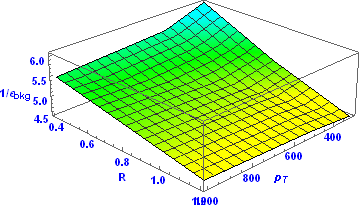
\includegraphics[width=0.30\textwidth]{./Figures/QGSurface/C11Tau11.png}}
\subfigure[$C_1^{\beta=2}+\tau_{1}^{\beta=2}$]{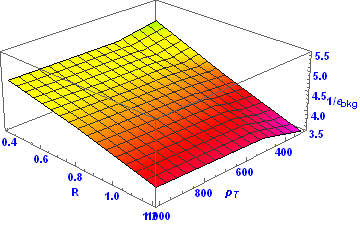
\includegraphics[width=0.30\textwidth]{./Figures/QGSurface/C12Tau12.png}}
%\subfigure[$C_1^{\beta=0}$]{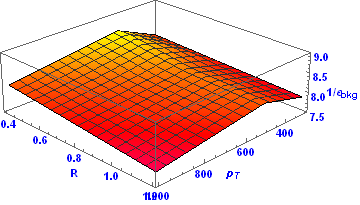
\includegraphics[width=0.30\textwidth]{./Figures/QGSurface/C10.png}}\\
%\subfigure[$C_1^{\beta=1}$]{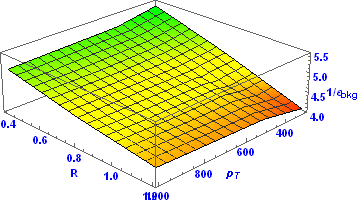
\includegraphics[width=0.30\textwidth]{./Figures/QGSurface/C11.png}}
%\subfigure[$\tau_{1}^{\beta=1}$]{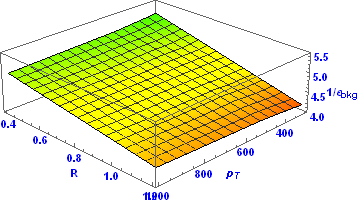
\includegraphics[width=0.30\textwidth]{./Figures/QGSurface/Tau11.png}}\\
%\subfigure[$C_1^{\beta=2}$]{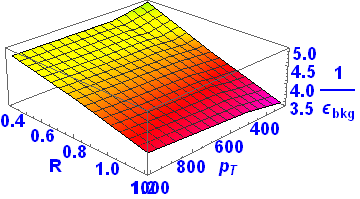
\includegraphics[width=0.30\textwidth]{./Figures/QGSurface/C12.png}}
%\subfigure[$\tau_{1}^{\beta=2}$]{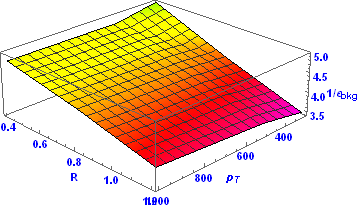
\includegraphics[width=0.30\textwidth]{./Figures/QGSurface/Tau12.png}}
%\subfigure[Ungroomed mass]{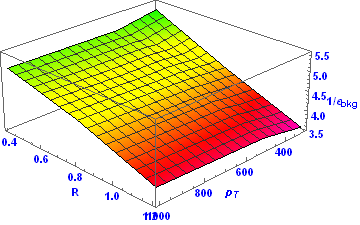
\includegraphics[width=0.30\textwidth]{./Figures/QGSurface/Mass.png}}\\
\caption{Surface plots of $1/\epsilon_\text{bkg}$ for the indicated pairs of variables from Classes IV and V considered for
  quark-gluon discrimination as functions of $R$ and $\pt$. }
\label{fig:qg_surface_pairA}
\end{figure*}
%


\subsection{Combined Performance and Correlations}\label{sec:qg_combi}
The quark/gluon tagging performance can be further improved over cuts on single observables by 
combining multiple observables in a BDT; due to the challenging nature of $q$/$g$-tagging, any
improvement in performance with multivariable techniques could be critical for certain analyses, and the 
improvement could be more substantial in data than the marginal benefit found in MC  and shown
in Fig.~\ref{fig:qg_pt300_single}.
 Furthermore, insight can be gained into the 
features allowing for quark/gluon discrimination if the origin of the improvement  is
understood. To quantitatively study this improvement, we build quark/gluon taggers from
every pair-wise combination of variables studied in the previous section for comparison
with the all-variable combination.  To illustrate the results achieved in this way we will exhibit the same sort 2D of
surface plots as in Figure~\ref{fig:qg_surface_single}.  Based on our discussion of the correlated properties
of observables within a single class, we expect little improvement in the rejection rate when combining observables from the same class
and substantial improvement when combining observables from different classes.  

Figure~\ref{fig:qg_surface_pairA} shows pairwise plots for (a) Class IV and (b) Class V.  Comparing to the corresponding plots
in Figure~\ref{fig:qg_surface_single} we see that combining $C_1^{\beta=1}+\tau_{1}^{\beta=1}$ provides a 
small improvement in the rejection rate of about 
10\% (0.5 out of 5) with essentially no change in the $R$ and $\pt$ dependence, while combining $C_1^{\beta=2}+\tau_{1}^{\beta=2}$   
yields a rejection rate that is essentially identical to the single observable rejection rate for all $R$ and $\pt$ values (with a similar conclusion if one
of these observables is replaced with the ungroomed jet mass $m$).  
This again confirms that expectation that the
observables within a single class effectively probe the \textit{same} jet properties.

 
%
\begin{figure*}
\centering
\subfigure[$\rm{N_ {constits}}+\Gamma_{Qjet}$]{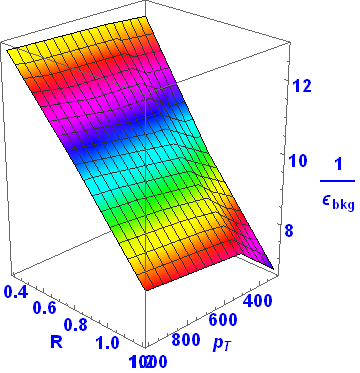
\includegraphics[width=0.28\textwidth]{./Figures/QGSurface/NconGamQ.png}}
\subfigure[$\rm{N_ {constits}}+ C_1^{\beta=1}$]{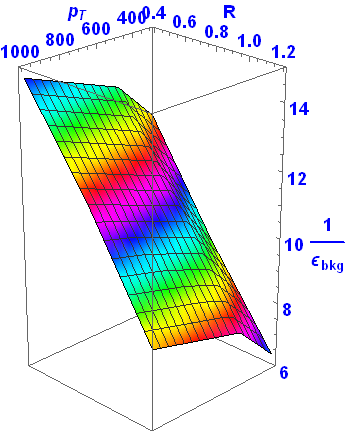
\includegraphics[width=0.28\textwidth]{./Figures/QGSurface/NconC11.png}}
\subfigure[$\rm{N_ {constits}}+ C_1^{\beta=2}$]{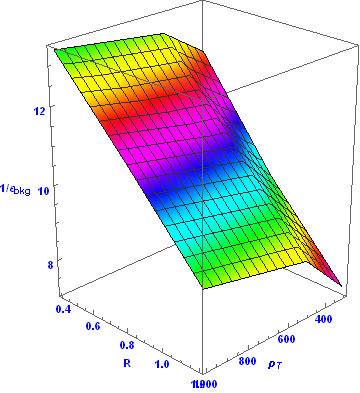
\includegraphics[width=0.28\textwidth]{./Figures/QGSurface/NconC12.png}}\\
\subfigure[$\rm{N_ {constits}}+ C_1^{\beta=0}$]{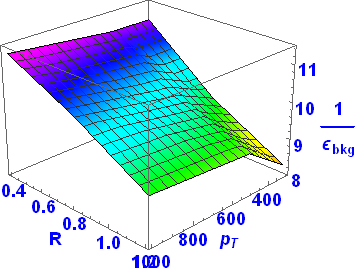
\includegraphics[width=0.28\textwidth]{./Figures/QGSurface/NconC10.png}}
\subfigure[$\Gamma_{Qjet}+ C_{1}^{\beta=0}$]{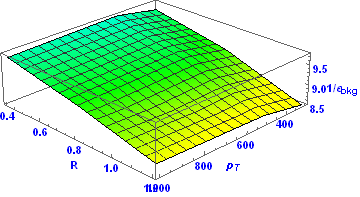
\includegraphics[width=0.28\textwidth]{./Figures/QGSurface/C10GamQ.png}}
\subfigure[$\Gamma_{Qjet}+ C_{1}^{\beta=1}$]{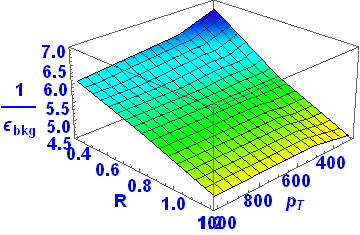
\includegraphics[width=0.28\textwidth]{./Figures/QGSurface/C11GamQ.png}}\\
\subfigure[$\Gamma_{Qjet}+ C_{1}^{\beta=2}$]{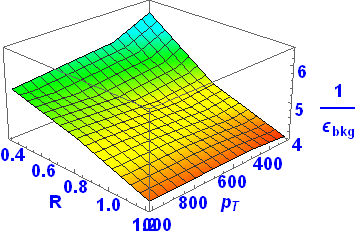
\includegraphics[width=0.28\textwidth]{./Figures/QGSurface/C12GamQ.png}}
\subfigure[$ C_{1}^{\beta=0}+ C_{1}^{\beta=1}$]{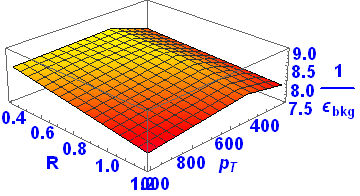
\includegraphics[width=0.28\textwidth]{./Figures/QGSurface/C10C11.png}}
\subfigure[$ C_{1}^{\beta=0}+ C_{1}^{\beta=2}$]{\includegraphics[width=0.28\textwidth]{./Figures/QGSurface/C10C12.png}}\\
\subfigure[$ C_{1}^{\beta=1}+ C_{1}^{\beta=2}$]{\includegraphics[width=0.28\textwidth]{./Figures/QGSurface/C11C12.png}}
\subfigure[All]{\includegraphics[width=0.28\textwidth]{./Figures/QGSurface/All.png}}
\caption{Surface plots of $1/\epsilon_\text{bkg}$ for the indicated pairs of variables from different classes considered for
  quark-gluon discrimination as functions of $R$ and $\pt$. }
\label{fig:qg_surface_pairB}
\end{figure*}
%

Next we consider the cross-class pairs of observables indicated in Figure~\ref{fig:qg_surface_pairB}, where only one member of
Classes IV and V is included.  As expected the largest rejection
rates are obtained from combining another observable with $\rm{N_ {constits}}$ (Figures~\ref{fig:qg_surface_pairB}(a) to (d)).  
In general, the rates are larger
than for the single variable case with similar $R$ and $\pt$ dependence.  In particular, the pair $\rm{N_ {constits}}+ C_1^{\beta=1}$ 
yields rejection rates in the range 6.4 to 14.7 (6.4 to 15 for the similar case $\rm{N_ {constits}}+ \tau_1^{\beta=1}$) with the largest
values at small $R$ and large $\pt$.  The other pairings with $\rm{N_ {constits}}$ (except with $\tau_1^{\beta=1}$) yield smaller 
rejection rates and smaller dynamic range.  The pair $\rm{N_ {constits}}+ C_1^{\beta=0}$ (Figure~\ref{fig:qg_surface_pairB}(d)) exhibits
the smallest range of rates (8.3 to 11.3) suggesting that the differences between these two observables serve to substantially 
reduce the $R$ and $\pt$ dependence for the pair, but this also reduces the possible optimization.  The other pairs indicated exhibit
similar behavior.  The pair rejection rates are somewhat better than either observable alone (since we are always combining from different classes),
and the $R$ and $\pt$ dependence is generally similar to the more variant single observable case.  The smallest $R$ and $\pt$ variation always occurs 
when pairing with $C_1^{\beta=0}$.  Changing any of the observables in these pairs with a different observable in the same class (\textit{e.g.},
$C_1^{\beta=2}$ for $\tau_1^{\beta=2}$ produces very similar results (at the few percent level).  Figure~\ref{fig:qg_surface_pairB}(k) shows the
result of a BDT analysis including all of the current observables with rejection rates in the range 10.5 to 17.1.  This is a somewhat narrower range
than in Figure~\ref{fig:qg_surface_pairB}(b) but with somewhat larger maximum values.

Another way to present the same data but by fixing $R$ and $\pt$ and showing all single observables and pairs of observables at once is in terms of the 
``matrices'' indicated in Figures~\ref{fig:qg_pt1000_comb} and \ref{fig:qg_akt4_comb}.  The numbers in each cell are the now familiar rejection factor
values of $1/\epsilon_\text{bkg}$ (gluons) for $\epsilon_\text{sig}= 50\,\% $ (quarks).  Figure~\ref{fig:qg_pt1000_comb} corresponds $\pt=1-1.1 \TeV$ and
$R =0.4,0.8,1.2$, while  Figure~\ref{fig:qg_akt4_comb} is for $R = 0.4$ and the 3 $\pt$ bins.  The actual numbers should be familiar from the discussion
above with the single observable rejections rates appearing on the diagonal and the pairwise results off the diagonal. 
The correlations indicated by the shading should be largely understood as indicating the organization of the observables into the now familiar
classes.  The all-observable (BDT) result appears as the number at the lower right in each plot.

%In order to quantitatively study the value of each variable for quark/gluon tagging, we study the gluon 
%rejection, defined as $1/\epsilon_{\rm gluon}$, at a fixed quark selection efficiency
%of 50\% using jets with $\pt=1-1.1 \TeV$ and for different $R$ parameters. Figure~\ref{fig:qg_pt1000_comb} shows the gluon 
%rejection for each pair-wise combination. 
%The pair-wise gluon rejection at 50\% quark efficiency can be compared to the single-variable
%values shown along the diagonal. The gluon rejection for the 
%BDT all-variable combination is also shown on the bottom right of each plot.

%
\begin{figure*}
\centering
\includegraphics[width=0.48\textwidth]{./Figures/QGTagging/pT1000/AKtR04/effBkg2D.png}
\includegraphics[width=0.48\textwidth]{./Figures/QGTagging/pT1000/AKtR08/effBkg2D.png}
\includegraphics[width=0.48\textwidth]{./Figures/QGTagging/pT1000/AKtR12/effBkg2D.png}
\caption{Gluon rejection defined as $1/\epsilon_{\rm gluon}$ when using each 2-variable combination 
as a tagger with 50\% acceptance for quark jets. Results are shown for
jets with $\pt=1-1.1 \TeV$ and
for (top left) $R=0.4$; (top right) $R=0.8$; (bottom) $R=1.2$. The rejection obtained with a tagger that uses all variables is also shown
in the plots. }
\label{fig:qg_pt1000_comb}
\end{figure*}
%

%As already observed in the previous section, $n_{\rm constits}$ is the most powerful single variable and
%$\C{1}{\beta=0}$ follows closely. However, the gains are largely correlated; the combined performance of $n_{\rm constits}$ and $\C{1}{\beta=0}$ is generally poorer than %combinations of $n_{\rm constits}$ with other jet substructure observables, such as $\tau_1$. Interestingly, in spite of the high correlation between $n_{\rm constits}$ and %$\C{1}{\beta=0}$, the two-variable combinations of $n_{\rm constits}$ generally fare worse than two-variable combinations with $\C{1}{\beta=0}$ . In particular,
%the combinations of $\tau^{\beta=1}_1$ or $\C{1}{\beta=1}$ with $n_{\rm constits}$ are capable of 
%getting very  close to the rejection achievable through the use of all variables for $R=0.4$ and $R=0.8$.

% Tagging of quark and gluon jets is generally better at small $R$. 
%The overall loss in performance
%with increasing $R$ can be seen in most single variables we study; this is expected, since more of the parton radiation is captured in the jet and more contamination from %underlying event occurs, suppressing the differences between $q$/$g$ jets. 
%The principal exceptions are $\C{1}{\beta=0}$ and 
%the Q-jet mass volatility, which are both quite resilient to increasing $R$. For $\C{1}{\beta=0}$, this is due to the fact that the exponent on $\Delta R$ is zero, and so soft %radiation at the periphery of the jet does not substantially change the distribution; as a result, the performance is largely independent of $R$.  Similarly, the soft radiation distant %from the jet centre will be vetoed during pruning regardless of the cluster sequence, and so the $R$-dependence of $\Gamma_{\rm Qjet}$ is not significant.   ({\bf BS: Check my %logic?}) Their combination, however, does perform slightly worse at larger $R$. ({\bf BS: I don't understand this, but it is a $\sim10\%$ effect, so maybe not too significant?}).
%By contrast, $\tau_1^{(\beta=2)}$ and $\C{1}{\beta=2}$
%are particularly sensitive to increasing R since, for $\beta=2$,
%large-angle emissions are given a larger weight. 

%These observations are qualitatively similar across all ranges of $\pt$. Quantitatively, however,
%there is a loss of rejection power for the taggers made of a combination of variables as the $\pt$ decreases. 
%This can be observed in Fig.~\ref{fig:qg_akt4_comb} for anti-$\kT$ R=0.4 jets of different $\pt$s. 
\begin{figure*}
\centering
\includegraphics[width=0.48\textwidth]{./Figures/QGTagging/pT300/AKtR04/effBkg2D.png}
%\includegraphics[width=0.4\textwidth]{./Figures/QGTagging/pT1000/AKtR04/Rocs_1D_single.png}\\
\includegraphics[width=0.48\textwidth]{./Figures/QGTagging/pT500/AKtR04/effBkg2D.png}
%\includegraphics[width=0.4\textwidth]{./Figures/QGTagging/pT1000/AKtR08/Rocs_1D_single.png}\\
\includegraphics[width=0.48\textwidth]{./Figures/QGTagging/pT1000/AKtR04/effBkg2D.png}
%\includegraphics[width=0.4\textwidth]{./Figures/QGTagging/pT1000/AKtR12/Rocs_1D_single.png}\\
\caption{Gluon rejection defined as $1/\epsilon_{\rm gluon}$ when using each 2-variable combination 
as a tagger with 50\% acceptance for quark jets. Results are shown for R=0.4 jets with (top left) $\pt=300-400 \GeV$, 
(top right) $\pt=500-600 \GeV$ and (bottom) $\pt=1-1.1 \TeV$. The rejection obtained with a tagger that uses all variables is also shown
in the plots. }
\label{fig:qg_akt4_comb}
\end{figure*}
%Clearly, most single variables retain their gluon rejection potential at lower $\pt$. However, when combined
%with other variables, the highest performing pairwise combinations lose ground with respect to other pairwise 
%combinations. This is also reflected in the rejection of the tagger that uses a combination of all variables, which
%is lower at lower $\pt$s. {\bf [do we understand this?]} ({\bf BS: This is a bit of a guess, but could it be that there is typically less radiation for low $\pt$, and so you're more %sensitive to fluctuations; since you have less access to information, combinations of observables perform less well than at high $\pt$.})




%\subsection{QJets Volatility and $\ptd$ ($\C{1}{\beta=0}$)}

%Simple explanation of correlation, or why does combining volatility and $\ptd$ improve quark versus gluon discrimination.  $\ptd$ ($\C{1}{\beta=0}$) takes small (large) values for a jet with near-democratic energy sharing between particles and large (small) values when the energy of the jet is contained in a few particles.  Because we expect gluons to radiate more particles, we expect that $\ptd_g<\ptd_q$ (or ${\C{1}{\beta=0}}_g>{\C{1}{\beta=0}}_q$).  Now, we expect the volatility of gluon jets to be in general smaller than that of quark jets because there is a greater probability (by a factor of about $C_A/C_F=9/4$) that there was a relatively hard emission in a jet that is not groomed away.  By measuring both volatility and $\ptd$, we are sensitive to both regions of phase space: where a relatively hard emission dominates the mass of the jet as well as the region where many soft emissions set the jet mass.


\subsection{QCD Jet Masses}\label{sec:qg_mass}

\begin{figure*}
\centering
\subfigure[Quark jets]{\includegraphics[width=0.40\textwidth]{./Figures/QGMass/m_quarks_log.png}}
\subfigure[Gluon jets]{\includegraphics[width=0.40\textwidth]{./Figures/QGMass/m_gluon_log.png}}
\caption{Comparisons of quark and gluon ungroomed mass distributions versus the scaled variable $m/p_T/R$. }
\label{fig:qg_masses_log}
\end{figure*}

To close the discussion of the tagging of jets as either quark jets or gluon jets we provide some insight into the behavior of the masses of such QCD jets,
both with and without grooming.  Recall that, in practice, an identified jet is simply a list of constituents, \textit{i.e.}, objects in the detector.  To the extent
that the masses of these individual constituents are irrelevant, typically because the detected constituents are relativistic, each constituent has a ``well''
defined 4-momentum.  It follows that the 4-momentum of the jet  is simply the sum of the 4-momenta of the constituents and its square is the jet mass squared.
We have already seen one set of jet mass distributions in  Figure~\ref{fig:qg_pt500_subst_AKt_R08}(h) for quark and gluon jets found with the anti-$\kT$
algorithm with  $R = 0.8$ and $\pt$ in the bin 500-600 GeV.  If we consider the mass distributions for other kinematic points (other values of $R$ and $\pt$),
we observe considerable variation but that variation can largely be removed by plotting versus the scaled variable $m/p_T/R$.  Simply on dimensional grounds
we know that jet mass must scale essentially linearly with $\pt$, with the remaining $\pt$ dependence arising predominantly from the running of the coupling,
$\alpha_s(\pt)$.  The $R$ dependence is also crudely linear as the mass scales approximately with the largest angular opening between any 2 constituents
and that is set by $R$.  The mass distributions for quark and gluon jets versus $m/p_T/R$ for all of our kinematic points 
are indicated in Figure~\ref{fig:qg_masses_log}, where
we use a logarithmic scale on the y-axis to clearly exhibit the behavior of these distributions over a large dynamic range.  We observe that the distributions
for the different kinematic points do approximately scale, \textit{i.e.}, the simple arguments above do capture most of the variation with $R$ and $\pt$.
We will consider shortly an explanation of the residual non-scaling. 

\begin{figure*}
\centering
\subfigure[Quark jets]{\includegraphics[width=0.40\textwidth]{./Figures/QGMass/mpr_quarks_log.png}}
\subfigure[Gluon jets]{\includegraphics[width=0.40\textwidth]{./Figures/QGMass/mpr_gluon_log.png}}
\caption{Comparisons of quark and gluon pruned mass distributions versus the scaled variable $m_\text{pr}/p_T/R$. }
\label{fig:qg_prmasses_log}
\end{figure*}

Several features of Figure~\ref{fig:qg_masses_log} can be easily understood.  The distributions all cut-off rapidly for $m/p_T/R > 0.5$, which is understood as
the precise limit (maximum mass) for a jet composed of just 2 constituents.  As expected from the soft and collinear singularities in QCD, the mass distribution peaks 
at small mass values.  The actual peak is ``pushed'' away from the origin by the so-called Sudakov form factor.  Summing the corresponding logarithmic structure 
(singular in both $\pt$ and angle) to all orders in perturbation theory yields a distribution that is highly damped  as the mass vanishes.  In words, there is precisely 
\textit{zero} probability that a color parton emits \textit{no} radiation (and the resulting jet has zero mass). 
 The large mass ``shoulder" ($0.3 < m/p_T/R < 0.5$) is driven largely by the presence of a single large angle, energetic
emission in the underlying QCD shower, \textit{i.e.}, this regime is quite well described by low-order perturbation theory. 
 (The shoulder label will be more clear after we groom the jet.)
In contrast, we should think of the peak region as corresponding to multiple soft emissions.  This simple (approximate) picture 
provides an understanding of the bulk of the
differences between the quark and gluon jet mass distributions.  Since the probability of the single large angle, energetic emission is proportional to the color charge,
the gluon distribution should be enhanced in this region by a factor of about $C_A/C_F = 9/4$, consistent with what is observed in Figure~\ref{fig:qg_masses_log}.
Similarly the exponent in the Sudakov damping factor for the gluon jet mass distribution  is enhanced by the same factor, 
leading to a peak ``pushed'' further from the origin.  So the gluon jet mass 
distribution exhibits a larger average jet mass than the quark jet, with a larger relative contribution arising from the perturbative shoulder region.  Recall also that
the number of constituents in the jet is also larger (on average) for the gluon jet simply because a gluon will radiate more than a quark.  
These features explain much of what we observed earlier in terms of the effectiveness of the various observable to separate quark jets from gluons jets.
Note in particular that the enhanced role of the shoulder for gluon jet explains, at least qualitatively, the difference in the distributions for the observable 
$\Gamma_{Qjet}$.  Since the shoulder is dominated by a single large angle, hard emission, ii is minimally impacted by pruning,
which removes the large angle, \textit{soft} constituents (as illustrated just below). Thus jets in the shoulder exhibit small volatility and they are a larger
component in the gluon jet distribution.  Hence gluon jets, on average, have smaller values of  $\Gamma_{Qjet}$ than quark jets as in 
Figure~\ref{fig:qg_pt500_subst_AKt_R08}(b).  Further this feature of gluon jets is distinct from fact that there are more constituents, which explains why
$\Gamma_{Qjet}$ and $\rm{N_ {constits}}$ supply largely independent information for distinguishing quark and gluon jets. 

To illustrate some of these points in more detail, Figure~\ref{fig:qg_prmasses_log} exhibits the jet mass distributions (of  Figure~\ref{fig:qg_masses_log}) 
\textit{after pruning}\cite{Ellis:2009me,Ellis:2009su}.  Removing the large angle,  soft constituents
moves the peak in both of the distributions from  $m/p_T/R \sim 0.1 - 0.2$ to the region around $m/p_T/R \sim 0.05$.  This explains why pruning works to reduce the
QCD background when looking for a signal in a specific jet mass bin.  The ``shoulder'' feature is much more apparent after pruning, as is the larger shoulder for
the gluon jets.  

Our final topic is the residual $R$ and $\pt$ dependence exhibited in Figures~\ref{fig:qg_masses_log} and \ref{fig:qg_prmasses_log}, where we are
using the scaled variable $m/p_T/R$.  As already suggested, the residual $\pt$ dependence can be understood as arising primarily from the slow decrease of the strong
coupling $\alpha_s(\pt)$ as $\pt$ increases.  This will lead to a corresponding decrease in the (largely perturbative) shoulder regime for both distributions
as $\pt$ increases.  At the same time, and for the same reason, the Sudakov damping is less strong with increasing $\pt$ and the peak moves towards the origin.
Thus the overall impact of increasing $\pt$ for both distributions is a (slow) shift to smaller values of $m/p_T/R$.  This is just what is observed in 
Figures~\ref{fig:qg_masses_log} and \ref{fig:qg_prmasses_log}, although the numerical size of the effect is reduced in the pruned case.
The $R$ dependence is more complicated as there are effectively three different contributions to the mass distribution.  
The perturbative large angle, energetic single emission contribution
largely scales in the variable $m/p_T/R$, which is why we see little residual $R$ dependence in either figure for $m/p_T/R > 0.4$.  
The large angle soft emissions can both contribute
at mass values that scale like $R$ and increase in number as $R$ increases (\textit{i.e.}, as the area of the jet grows as $R^2$).  Such contributions can yield
a distribution that moves to the right as $R$ increases and presumably explain the behavior at small $\pt$ in Figure~\ref{fig:qg_masses_log}.  Since pruning
largely removes this contribution, we observe no such behavior in Figure~\ref{fig:qg_prmasses_log}.  The contribution of small angle, soft emissions will be at
fixed $m$ values and thus shift to the left versus the scaled variable as $R$ increases.  
This presumably explains the small shifts in this direction observed in both figures.

 \subsection{Conclusions}\label{sec:qg_concl}

In Section~\ref{sec:qgtagging} we have seen that a variety of jet observables
 provide information about the jet that can be employed effectively to separately tag quark and gluon jets.  Further,
when used in combination, these observables can provide even better separation.  We saw that the best performing single observable is simply the number of
constituents in the jet, $\rm{N_ {constits}}$,  while the largest further improvement comes from combining with $C_1^{\beta =1}$ (or $\tau_1^{\beta=1}$), 
but the smallest
$R$ and $\pt$ dependence arises from combining with $C_1^{\beta = 0}$.  On the other hand, some of the commonly used observables are highly correlated
and do not provide extra information and enhanced tagging when used together.  We have both demonstrated these correlations and provided a discussion of the 
physics behind the structure of the correlation.  In particular, using the jet mass as a specific example observable we have tried to explicitly explain the differences between jets 
initiated by both quarks and gluons. 
 